% Options for packages loaded elsewhere
\PassOptionsToPackage{unicode}{hyperref}
\PassOptionsToPackage{hyphens}{url}
%
\documentclass[
]{book}
\usepackage{amsmath,amssymb}
\usepackage{lmodern}
\usepackage{iftex}
\ifPDFTeX
  \usepackage[T1]{fontenc}
  \usepackage[utf8]{inputenc}
  \usepackage{textcomp} % provide euro and other symbols
\else % if luatex or xetex
  \usepackage{unicode-math}
  \defaultfontfeatures{Scale=MatchLowercase}
  \defaultfontfeatures[\rmfamily]{Ligatures=TeX,Scale=1}
\fi
% Use upquote if available, for straight quotes in verbatim environments
\IfFileExists{upquote.sty}{\usepackage{upquote}}{}
\IfFileExists{microtype.sty}{% use microtype if available
  \usepackage[]{microtype}
  \UseMicrotypeSet[protrusion]{basicmath} % disable protrusion for tt fonts
}{}
\makeatletter
\@ifundefined{KOMAClassName}{% if non-KOMA class
  \IfFileExists{parskip.sty}{%
    \usepackage{parskip}
  }{% else
    \setlength{\parindent}{0pt}
    \setlength{\parskip}{6pt plus 2pt minus 1pt}}
}{% if KOMA class
  \KOMAoptions{parskip=half}}
\makeatother
\usepackage{xcolor}
\IfFileExists{xurl.sty}{\usepackage{xurl}}{} % add URL line breaks if available
\IfFileExists{bookmark.sty}{\usepackage{bookmark}}{\usepackage{hyperref}}
\hypersetup{
  pdftitle={Data Science with R (PSYC3012)},
  hidelinks,
  pdfcreator={LaTeX via pandoc}}
\urlstyle{same} % disable monospaced font for URLs
\usepackage{color}
\usepackage{fancyvrb}
\newcommand{\VerbBar}{|}
\newcommand{\VERB}{\Verb[commandchars=\\\{\}]}
\DefineVerbatimEnvironment{Highlighting}{Verbatim}{commandchars=\\\{\}}
% Add ',fontsize=\small' for more characters per line
\usepackage{framed}
\definecolor{shadecolor}{RGB}{248,248,248}
\newenvironment{Shaded}{\begin{snugshade}}{\end{snugshade}}
\newcommand{\AlertTok}[1]{\textcolor[rgb]{0.94,0.16,0.16}{#1}}
\newcommand{\AnnotationTok}[1]{\textcolor[rgb]{0.56,0.35,0.01}{\textbf{\textit{#1}}}}
\newcommand{\AttributeTok}[1]{\textcolor[rgb]{0.77,0.63,0.00}{#1}}
\newcommand{\BaseNTok}[1]{\textcolor[rgb]{0.00,0.00,0.81}{#1}}
\newcommand{\BuiltInTok}[1]{#1}
\newcommand{\CharTok}[1]{\textcolor[rgb]{0.31,0.60,0.02}{#1}}
\newcommand{\CommentTok}[1]{\textcolor[rgb]{0.56,0.35,0.01}{\textit{#1}}}
\newcommand{\CommentVarTok}[1]{\textcolor[rgb]{0.56,0.35,0.01}{\textbf{\textit{#1}}}}
\newcommand{\ConstantTok}[1]{\textcolor[rgb]{0.00,0.00,0.00}{#1}}
\newcommand{\ControlFlowTok}[1]{\textcolor[rgb]{0.13,0.29,0.53}{\textbf{#1}}}
\newcommand{\DataTypeTok}[1]{\textcolor[rgb]{0.13,0.29,0.53}{#1}}
\newcommand{\DecValTok}[1]{\textcolor[rgb]{0.00,0.00,0.81}{#1}}
\newcommand{\DocumentationTok}[1]{\textcolor[rgb]{0.56,0.35,0.01}{\textbf{\textit{#1}}}}
\newcommand{\ErrorTok}[1]{\textcolor[rgb]{0.64,0.00,0.00}{\textbf{#1}}}
\newcommand{\ExtensionTok}[1]{#1}
\newcommand{\FloatTok}[1]{\textcolor[rgb]{0.00,0.00,0.81}{#1}}
\newcommand{\FunctionTok}[1]{\textcolor[rgb]{0.00,0.00,0.00}{#1}}
\newcommand{\ImportTok}[1]{#1}
\newcommand{\InformationTok}[1]{\textcolor[rgb]{0.56,0.35,0.01}{\textbf{\textit{#1}}}}
\newcommand{\KeywordTok}[1]{\textcolor[rgb]{0.13,0.29,0.53}{\textbf{#1}}}
\newcommand{\NormalTok}[1]{#1}
\newcommand{\OperatorTok}[1]{\textcolor[rgb]{0.81,0.36,0.00}{\textbf{#1}}}
\newcommand{\OtherTok}[1]{\textcolor[rgb]{0.56,0.35,0.01}{#1}}
\newcommand{\PreprocessorTok}[1]{\textcolor[rgb]{0.56,0.35,0.01}{\textit{#1}}}
\newcommand{\RegionMarkerTok}[1]{#1}
\newcommand{\SpecialCharTok}[1]{\textcolor[rgb]{0.00,0.00,0.00}{#1}}
\newcommand{\SpecialStringTok}[1]{\textcolor[rgb]{0.31,0.60,0.02}{#1}}
\newcommand{\StringTok}[1]{\textcolor[rgb]{0.31,0.60,0.02}{#1}}
\newcommand{\VariableTok}[1]{\textcolor[rgb]{0.00,0.00,0.00}{#1}}
\newcommand{\VerbatimStringTok}[1]{\textcolor[rgb]{0.31,0.60,0.02}{#1}}
\newcommand{\WarningTok}[1]{\textcolor[rgb]{0.56,0.35,0.01}{\textbf{\textit{#1}}}}
\usepackage{longtable,booktabs,array}
\usepackage{calc} % for calculating minipage widths
% Correct order of tables after \paragraph or \subparagraph
\usepackage{etoolbox}
\makeatletter
\patchcmd\longtable{\par}{\if@noskipsec\mbox{}\fi\par}{}{}
\makeatother
% Allow footnotes in longtable head/foot
\IfFileExists{footnotehyper.sty}{\usepackage{footnotehyper}}{\usepackage{footnote}}
\makesavenoteenv{longtable}
\usepackage{graphicx}
\makeatletter
\def\maxwidth{\ifdim\Gin@nat@width>\linewidth\linewidth\else\Gin@nat@width\fi}
\def\maxheight{\ifdim\Gin@nat@height>\textheight\textheight\else\Gin@nat@height\fi}
\makeatother
% Scale images if necessary, so that they will not overflow the page
% margins by default, and it is still possible to overwrite the defaults
% using explicit options in \includegraphics[width, height, ...]{}
\setkeys{Gin}{width=\maxwidth,height=\maxheight,keepaspectratio}
% Set default figure placement to htbp
\makeatletter
\def\fps@figure{htbp}
\makeatother
\setlength{\emergencystretch}{3em} % prevent overfull lines
\providecommand{\tightlist}{%
  \setlength{\itemsep}{0pt}\setlength{\parskip}{0pt}}
\setcounter{secnumdepth}{5}
\usepackage{booktabs}
\usepackage{booktabs}
\usepackage{longtable}
\usepackage{array}
\usepackage{multirow}
\usepackage{wrapfig}
\usepackage{float}
\usepackage{colortbl}
\usepackage{pdflscape}
\usepackage{tabu}
\usepackage{threeparttable}
\usepackage{threeparttablex}
\usepackage[normalem]{ulem}
\usepackage{makecell}
\usepackage{xcolor}
\ifLuaTeX
  \usepackage{selnolig}  % disable illegal ligatures
\fi
\usepackage[]{natbib}
\bibliographystyle{plainnat}

\title{Data Science with R (PSYC3012)}
\usepackage{etoolbox}
\makeatletter
\providecommand{\subtitle}[1]{% add subtitle to \maketitle
  \apptocmd{\@title}{\par {\large #1 \par}}{}{}
}
\makeatother
\subtitle{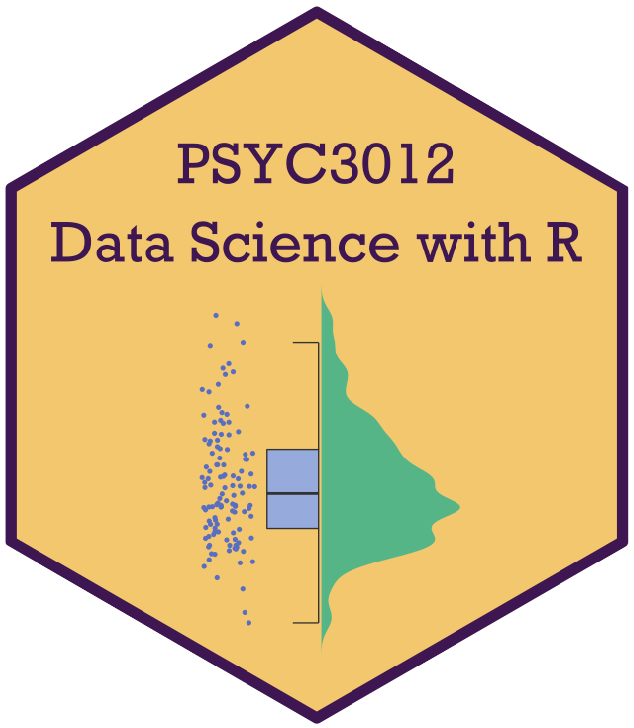
\includegraphics[width=3in,height=\textheight]{images/psyc3012_hex.png}}
\author{true \and true \and true}
\date{}

\usepackage{amsthm}
\newtheorem{theorem}{Theorem}[chapter]
\newtheorem{lemma}{Lemma}[chapter]
\newtheorem{corollary}{Corollary}[chapter]
\newtheorem{proposition}{Proposition}[chapter]
\newtheorem{conjecture}{Conjecture}[chapter]
\theoremstyle{definition}
\newtheorem{definition}{Definition}[chapter]
\theoremstyle{definition}
\newtheorem{example}{Example}[chapter]
\theoremstyle{definition}
\newtheorem{exercise}{Exercise}[chapter]
\theoremstyle{definition}
\newtheorem{hypothesis}{Hypothesis}[chapter]
\theoremstyle{remark}
\newtheorem*{remark}{Remark}
\newtheorem*{solution}{Solution}
\begin{document}
\maketitle

{
\setcounter{tocdepth}{1}
\tableofcontents
}
\hypertarget{introduction}{%
\chapter*{Introduction}\label{introduction}}
\addcontentsline{toc}{chapter}{Introduction}

\textbf{Data Science with R} (PSYC3012) is a 15-credit optional module that aims to develop students' research skills relying on three main themes: Open Science, digital literacy, and science communication.

The module covers data wrangling, data visualization, categorical data analysis, general linear models, and robust statistics using R---a free software environment for statistical computing and graphics. Each session is grounded in Open Science best practices to favor reproducibility and transparency in science, following the guidelines of the 2019 Concordat to Support Research Integrity, the UK Reproducibility Network, and the 2016 Concordat on Open Research Data.

Upon successful completion of this module, students should be able to:

\begin{itemize}
\tightlist
\item
  Recognize, explain, and apply open science best practices following the Concordat on Open Research Data and the UK Reproducibility Network guidelines.
\item
  Identify and describe the appropriate analytical procedures required to answer research questions related to categorical data analysis and general linear models.
\item
  Apply R to organize and tidy the data, to model the data, and to generate appropriate data visualizations.
\item
  Inspect and appraise the outputs generated with R to produce with Rmarkdown a reproducible research report that will communicate the results relying on the principles of transparency and reproducibility in science.
\end{itemize}

\hypertarget{how-to-use-this-book}{%
\section*{How to use this book}\label{how-to-use-this-book}}
\addcontentsline{toc}{section}{How to use this book}

This book is intended to be the handbook of the optional module \textbf{Data Science with R} (PSYC3012); a module delivered for the Psychology undergraduate provisions at De Montfort University (Leicester, United Kingdom). This book includes all the content and reproducible examples that will be delivered in the 2-hour weekly sessions (Term 1, Academic Year 2023-24).

It is recommended to read in advance the corresponding chapters and sections that will be explained in class. Similarly, it is recommended to install \textbf{R}, \textbf{RStudio}, and the required R packages to work on the examples of this book before attending the first lecture and workshop. Please, read the software installation guidelines before reading the book (Appendix \ref{appenA}).

\hypertarget{about-the-author}{%
\section*{About the Author}\label{about-the-author}}
\addcontentsline{toc}{section}{About the Author}

\href{https://www.dmu.ac.uk/about-dmu/academic-staff/health-and-life-sciences/carlos-crivelli/carlos-crivelli.aspx}{Dr Carlos Crivelli} is an Associate Professor/Reader in Affective Science and Social Interaction in the School of Applied Social Sciences at De Montfort University (Leicester, United Kingdom).

After completing a BSc (Hons) Psychology, Dr Crivelli received his MSc and PhD in Methodology of Behavioral and Health Sciences from Universidad Autónoma de Madrid (Madrid, Spain). His research interests focus on three main areas: social influence and emotion science, cross-cultural psychology, and data science. He has published on these topics in journals like \href{https://www.cell.com/trends/cognitive-sciences/fulltext/S1364-6613(18)30029-9}{\emph{Trends in the Cognitive Sciences}}, \href{https://www.pnas.org/doi/full/10.1073/pnas.1611622113}{\emph{Proceedings of the National Academy of Sciences, U.S.A.}}, \href{https://journals.sagepub.com/doi/10.1177/17456916221148142}{\emph{Perspectives on Psychological Science}}, and \href{https://journals.sagepub.com/doi/full/10.1177/0963721417746794}{\emph{Current Directions in Psychological Science}}.

Dr.~Crivelli is an Honorary Fellow of the University of Melbourne (Australia), a Fellow of the Higher Education Academy, and a member of the editorial board of \href{https://www.nature.com/sdata/}{\emph{Nature--Scientific Data}}. He teaches undergraduate and postgraduate courses in Psychometrics and Data Science in R, Personality and Intelligence, and Conceptual Issues and Critical Debates in Psychology, embedding the intercultural dimension, and open and reproducible research into the curriculum.

\hypertarget{what-is-open-science}{%
\chapter{What is Open Science?}\label{what-is-open-science}}

\begin{quote}
\textbf{LEARNING OUTCOMES}

\begin{itemize}
\tightlist
\item
  Identify and explain Open Science's principles.
\item
  Compare the different initiatives promoting Open Science nationally and internationally.
\item
  Appraise the implications of using Open Science's principles of reproducibility, openness, and replicability in the research process.
\item
  Apply Open Science to comply with the regulations of research institutions and funders, governments, and publishers.
\item
  Identify the steps required and implement the best practices to promote data sharing, open code and software, and data curation.
\end{itemize}
\end{quote}

According to the 2021 United Nations Educational, Scientific and Cultural Organization (UNESCO) Recommendation on Open Science, ``\ldots{} \textbf{Open Science} is defined as an inclusive construct that combines various movements and practices aiming to make multilingual scientific knowledge openly available, accessible and reusable for everyone, to increase scientific collaborations and sharing of information for the benefits of science and society, and to open the processes of scientific knowledge creation, evaluation and communication to societal actors beyond the traditional scientific community. It comprises all scientific disciplines and aspects of scholarly practices, including basic and applied sciences, natural and social sciences and the humanities, and it builds on the following key pillars: open scientific knowledge, open science infrastructures, science communication open engagement o societal actors and open dialogue with other knowledge systems.'' (2017, p.~7)

For The European Commission's task force on Research and Innovation (2021), ``\textbf{Open Science} is a system change allowing for better science through open and collaborative ways of producing and sharing knowledge and data, as early as possible in the research process, and for communicating and sharing results. This new approach affects research institutions and science practices by bringing about new ways of funding, evaluating, and rewarding researchers. Open Science increases the quality and impact of science by fostering reproducibility and interdisciplinarity. It makes science more efficient through better sharing of resources, more reliable through better verification and more responsive to society's needs'' (p.~1)

In the United Kingdom, different regulations on open science (also named \emph{Open Research} or \emph{Open Scholarship}) has been developed. For example, the \href{https://www.universitiesuk.ac.uk/topics/research-and-innovation/concordat-support-research-integrity}{2019 Concordat to Support Research Integrity (Universities UK)} or the \href{https://www.ukri.org/wp-content/uploads/2020/10/UKRI-020920-ConcordatonOpenResearchData.pdf}{2016 Concordat on Open Research Data (HEFCE, Research Councils UK, Wellcome Trust, Universities UK)} have captured some of the initiatives on Open Science discussed and developed by other policy makers, institutions, publishers, funders, and research councils. It is important to note that the \href{https://www.ukrn.org}{UK Reproducibility Network}---supported by UK Research Institute, the British Psychological Society, Wellcome Trust, Cancer Research UK, UK Data Service, or Universities UK---has played a pivotal role in ``seeking to understand the factors that contribute to poor research reproducibility and replicability, and to develop approaches to counter these and improve the quality of the research we produce'' (UK Reproducibility Network, 2021, p.~1).

\textbf{Open Science}

\textbf{Open Science} is a broad term used to encompass the promotion of \emph{transparency}, \emph{reproducibility}, \emph{research integrity}, and \emph{societal impact (research and innovation)}.

Because of those principles, \textbf{Open Science} can be reconceived as a meta-scientific movement interested in enhancing the following skills:

Digital content creation

Science communication

Information and data literacy

To empower researchers at every career stage, different organizations and Higher Education institutions have launched innovative educational programes along with institutional statements and strategies to promote Open Science best practices. For example, \href{https://www.sheffield.ac.uk/openresearch/university-statement-open-research}{the University of Sheffield} has launched an Open Science strategy to promote a culture of research excellence. \href{https://www.openresearch.manchester.ac.uk}{The University of Manchester} has created the Office for Open Research led big five strategic priorities: (1) open research skills, (2) open research communities, (3) open research recognition, (4) open research workflows, and (5) open and FAIR research outputs. Similarly, \href{https://www.surrey.ac.uk/sites/default/files/2022-02/open-research-strategic-goals-and-action-plan-2019-2024.pdf}{the University of Surrey} developed a 5-year open research strategic goals and action plan that emphasizes the awareness, training and advocacy of open practice across the university in research, teaching, and learning.

In December 2021, \href{https://repository.lboro.ac.uk/articles/online_resource/Loughborough_University_Open_Research_Position_Statement/11709975}{Loughborough University} published an Open Research Position Statement to develop, review, and promote an institutional policy framework for Open Research. Echoing the University of Manchester's strategic priorities, Loughborough University has emphasized the pivotal role of training and support for PhD students and senior academics to update their skills for open data and open methods (i.e., science communication, information and data literacy). Other universities stressing the importance of mastering digital literacy skills for open data and code/software (e.g., programming in R/Python, data sharing) are the Open Research Skills Framework at \href{https://subjectguides.york.ac.uk/openresearch}{the University of York}, \href{https://www.kcl.ac.uk/research/kings-open-research-group-initiative-korgi}{King's College} and their Open Research Group Initiative (KORGI), \href{https://www.gla.ac.uk/myglasgow/openresearch/}{the University of Glasgow}, the Reproducible Research Oxford group (RROx) at the \href{https://www.ox.ac.uk/research/support-researchers/open-research}{University of Oxford}, the Birmingham Environment for Academic Research's (BEAR) software carpentry training (in R, Python, Matlab, and Git) at \href{https://intranet.birmingham.ac.uk/it/teams/infrastructure/research/bear/index.aspx}{the University of Birmingham}, Open Research education for doctoral students at \href{https://www.imperial.ac.uk/research-and-innovation/support-for-staff/scholarly-communication/open-research/open-research-education/}{Imperial College London}, or the Edinburgh Open Research Initiative of \href{https://www.ed.ac.uk/information-services/about/organisation/library-and-collections/open-research/eori}{the University of Edinburgh}.

\begin{table}

\caption{\label{tab:Table11b}Open Science Skills and Required Training}
\centering
\resizebox{\linewidth}{!}{
\fontsize{14}{16}\selectfont
\begin{tabular}[t]{ll}
\toprule
\cellcolor[HTML]{EFEFEF}{Skills} & \cellcolor[HTML]{EFEFEF}{Training}\\
\midrule
\cellcolor[HTML]{E1FAFF}{Digital content creation} & \cellcolor[HTML]{E1FAFF}{Copyright and intellectual property (CC-BY)}\\
\cellcolor[HTML]{E1FAFF}{} & \cellcolor[HTML]{E1FAFF}{Management and use of institutional repositories (DORA)}\\
\cellcolor[HTML]{E1FAFF}{} & \cellcolor[HTML]{E1FAFF}{OA publishers (e.g., bookdown)}\\
\cellcolor[HTML]{E1FAFF}{} & \cellcolor[HTML]{E1FAFF}{Open publication options (e.g., Gold, Green)}\\
\cellcolor[HTML]{E1FAFF}{} & \cellcolor[HTML]{E1FAFF}{Data repositories (OSF, Zotero, Figshare, Github)}\\
\cellcolor[HTML]{E1FAFF}{} & \cellcolor[HTML]{E1FAFF}{Data management plan}\\
\cellcolor[HTML]{E1FAFF}{} & \cellcolor[HTML]{E1FAFF}{Data presentation}\\
\cellcolor[HTML]{D1FFEC}{Science communication} & \cellcolor[HTML]{D1FFEC}{Bibliometrics, Altmetrics, and researcher impact}\\
\cellcolor[HTML]{D1FFEC}{} & \cellcolor[HTML]{D1FFEC}{DMU/Institutional webpage}\\
\cellcolor[HTML]{D1FFEC}{} & \cellcolor[HTML]{D1FFEC}{Personal brand (e.g., ORCID, Researchgate, Google scholar, Scopus)}\\
\cellcolor[HTML]{D1FFEC}{} & \cellcolor[HTML]{D1FFEC}{Public engagement (e.g., Leicester Business Festival)}\\
\cellcolor[HTML]{D1FFEC}{} & \cellcolor[HTML]{D1FFEC}{Research informs teaching (handbooks, monographs, tutorials)}\\
\cellcolor[HTML]{D1FFEC}{} & \cellcolor[HTML]{D1FFEC}{Innovation (e.g., the role of visual statistics during COVID-19)}\\
\cellcolor[HTML]{FFF4D1}{Information and data literacy} & \cellcolor[HTML]{FFF4D1}{Data analysis and visualization}\\
\cellcolor[HTML]{FFF4D1}{} & \cellcolor[HTML]{FFF4D1}{Data wrangling, modeling}\\
\cellcolor[HTML]{FFF4D1}{} & \cellcolor[HTML]{FFF4D1}{Text mining (qualitative research)}\\
\cellcolor[HTML]{FFF4D1}{} & \cellcolor[HTML]{FFF4D1}{Secondary sources (e.g., spatial data, census)}\\
\cellcolor[HTML]{FFF4D1}{} & \cellcolor[HTML]{FFF4D1}{Reproducibility and data reuse}\\
\cellcolor[HTML]{FFF4D1}{} & \cellcolor[HTML]{FFF4D1}{Publish in data journals}\\
\cellcolor[HTML]{FFF4D1}{} & \cellcolor[HTML]{FFF4D1}{Transparency}\\
\cellcolor[HTML]{FFF4D1}{} & \cellcolor[HTML]{FFF4D1}{Research integrity}\\
\bottomrule
\end{tabular}}
\end{table}

\hypertarget{the-credibility-of-science}{%
\section{The credibility of Science}\label{the-credibility-of-science}}

The academic/research career runs in parallel with a cycle of credibility in which trust and reliability are sought (Miedema, 2022) (Figure 1.1).

To conduct any research project, we need staff (at least, one researcher) and equipment. Then, we need to design a research proposal and collect data. The data needs to be properly analyzed, requiring a set of research skills that enabled researchers to design the research proposal first, to collect data ensuring proper levels of quality and rigor, and the necessary skills to describe, model, visualize, and interpret the findings. The findings are supported by arguments (some of them are theoretical, whereas others are methodological) and often presented as a manuscript or research report. However, to publish those manuscripts and research reports, researchers need to demonstrate appropriate and highly valued research skills (e.g., deep knowledge of the theoretical approaches and literature review, critical evaluation skills, understanding of the methods and data analytical techniques used), not only to create those products for internal consumption, but to be accepted by the scientific community after passing the judgment of senior and experts peers (the peer-review system).

Once the products of our research are published, different metrics are used to provide the context of the quality of the research process. Metrics such as the Journal Citation Report impact factors, H-index, Google Scholar metrics, or Altmetrics are used for recognition and are a proxy to secure or increase the chances to secure funding, a good research/academic job, promotions, or to accrue more equipment and staff (e.g., research associates, post-docs, PhD students).

\begin{figure}

{\centering 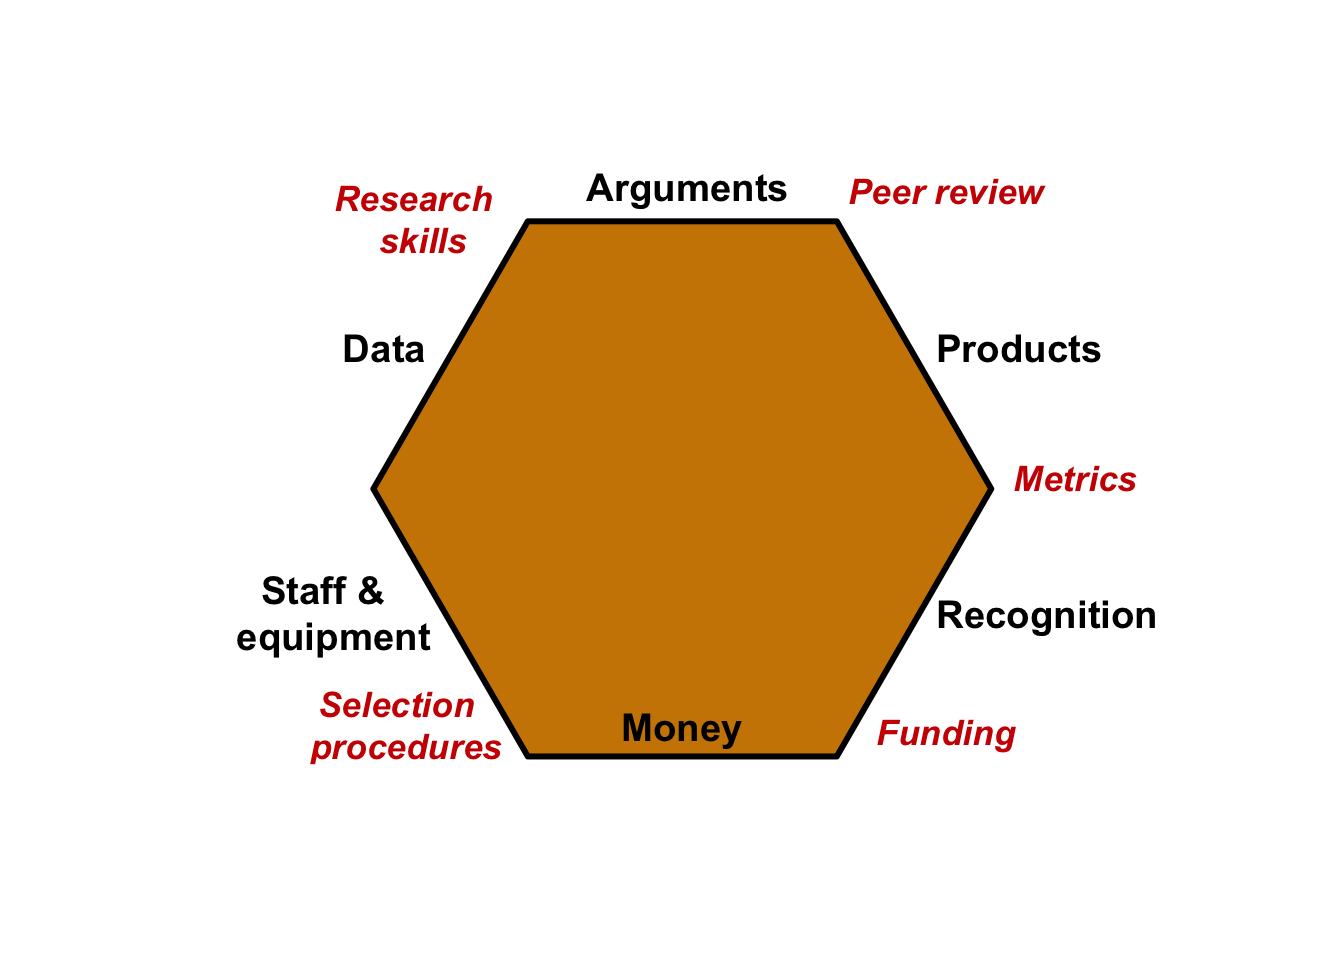
\includegraphics[width=1\linewidth]{_main_files/figure-latex/credibility-1} 

}

\caption{The credibility cycle}\label{fig:credibility}
\end{figure}

\hypertarget{questionable-scientific-practices}{%
\section{Questionable scientific practices}\label{questionable-scientific-practices}}

In the 2010s, disciplines such as psychology, economics, or the biomedical sciences were engulfed by a turmoil of distrust and lack of credibility. Although the Open Science movement is not new and it is at the core of the scientific method, a scientific reform movement emerged to inform on questionable scientific practices (John, Loewenstein, \& Prelec, 2012). Synchronically, a heated debate emerged to find solutions to the credibility crisis; a crisis that was triggered by the lack of openness, transparency, and replicability (Spellman et al., 2017).

\textbf{Questionable Scientific Practices}

Failing to report all dependent measures

Collecting more data after seeing whether results were significant

Failing to report all conditions

Stopping collecting data earlier than planned because one found the result that one had been looking for

Rounding down \emph{p} values selectively reporting

Selectively reporting studies that ``worked''

Excluding data after looking at the impact of doing so

Reporting an unexpected finding as having been predicted from the start

Falsely claiming that results are unaffected by demographic variables (e.g., gender) when one is unsure (or knows that they do)

Falsifying data

\begin{figure}

{\centering 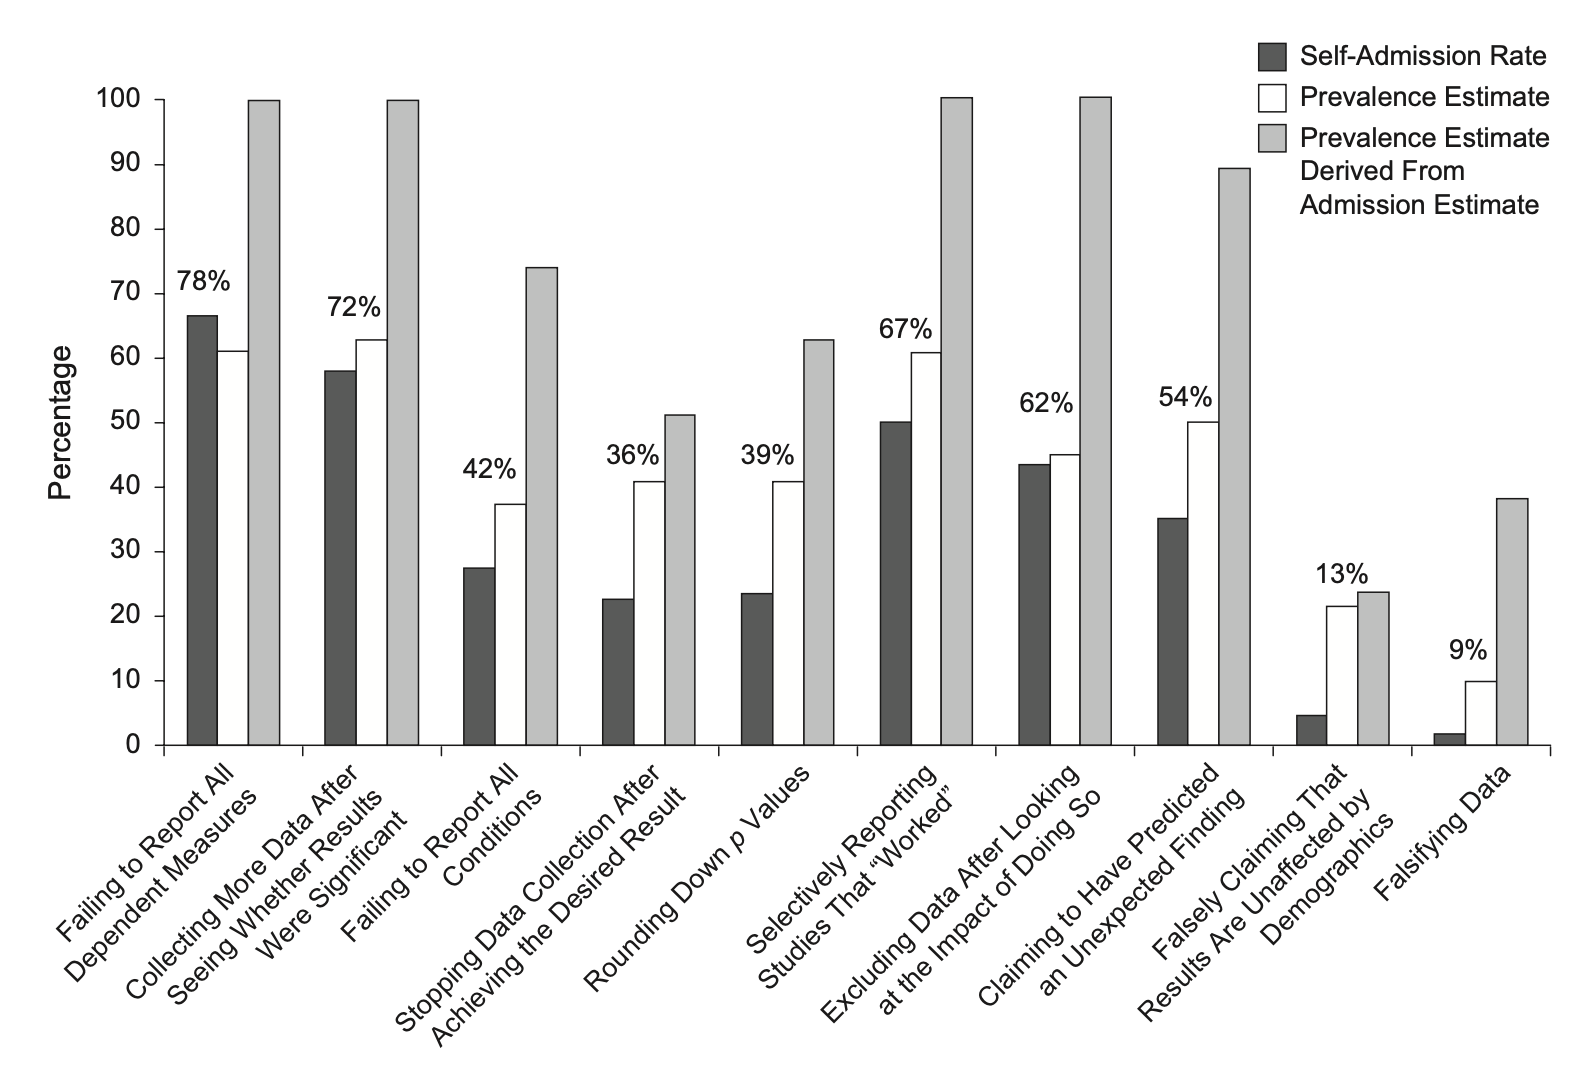
\includegraphics[width=0.95\linewidth]{./images/pqrpractice} 

}

\caption{Prevalence of questionable research practices (John, Loewenstein, $\&$ Prelec, 2012)}\label{fig:questionable}
\end{figure}

\hypertarget{the-credibility-crisis}{%
\section{The credibility crisis}\label{the-credibility-crisis}}

One of the most cited papers of the last decade (7,243 citations in January 2023) (Open Science Collaboration, 2015) conducted a large-scale study in which 100 classic psychological experiments were put to a test using an international, multi-lab approach. The main goal of the study was to estimate the reproducibility of psychological science. Unfortunately, the results showed that most of the classic psychological studies that psychology students learn in college and that most researchers cite as settled science couldn't be replicated. This meta-scientific endeavor has been conducted with similar results in other fields such as the behavioral, cognitive, economic, health, and medical sciences.

The most telling results showed that:

\begin{itemize}
\tightlist
\item
  psychologists tend to use under-powered samples that overestimate the effect size and produce low reproducibility of results
\item
  there is a lack of access to full methods
\item
  there is a lack of access to analytic procedures and code
\item
  the file-drawer problem is pervasive as editors and journals are keen to ``find results'' (i.e., rejection of the Null Hypothesis, rather that publish reports with null effects)
\item
  there is a lack of access to publications
\item
  there is discontent with reporting and use of standard statistics
\end{itemize}

\begin{figure}

{\centering 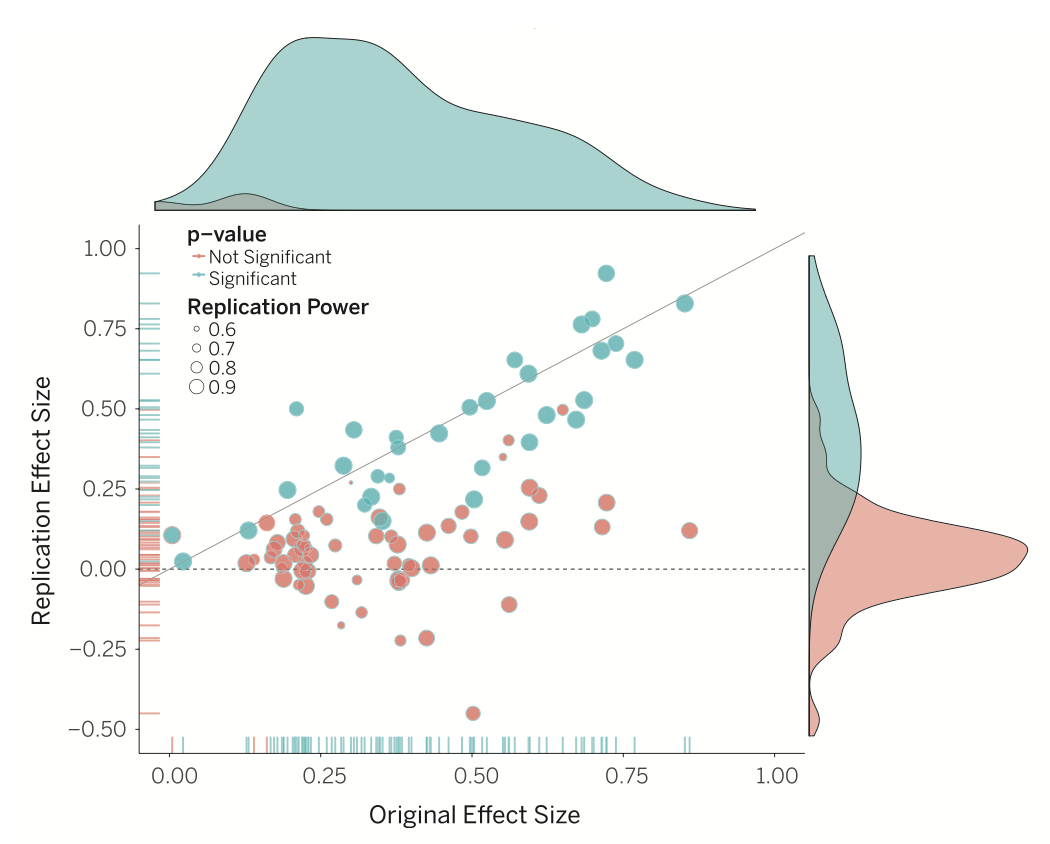
\includegraphics[width=0.9\linewidth]{./images/replic} 

}

\caption{Reproducibility of psychological science (Open Science Collaboration, 2015)}\label{fig:replication1}
\end{figure}

\hypertarget{threats-to-the-quality-of-the-scientific-process}{%
\section{Threats to the quality of the scientific process}\label{threats-to-the-quality-of-the-scientific-process}}

Kovacs and colleagues (2021) conducted a research project to elucidate the origins and causes of the most frequent mistakes committed by researchers that damaged the quality of the scientific process. Using a mix of quantitative and qualitative approaches to data collection, they surveyed 488 researchers publishing in psychology journals between 2010 and 2018. They found four supra-ordinal categories or metagroups and their corresponding causes (Table 1.2).

\begin{table}

\caption{\label{tab:Table12b}Metagroups for Mistake Causes}
\centering
\resizebox{\linewidth}{!}{
\fontsize{14}{16}\selectfont
\begin{tabular}[t]{ll}
\toprule
\cellcolor[HTML]{EFEFEF}{Metagroup} & \cellcolor[HTML]{EFEFEF}{Cause group}\\
\midrule
\cellcolor[HTML]{E1FAFF}{Poor project preparation or management} & \cellcolor[HTML]{E1FAFF}{Bad or lack of planning}\\
\cellcolor[HTML]{E1FAFF}{} & \cellcolor[HTML]{E1FAFF}{Bad or lack of standards}\\
\cellcolor[HTML]{E1FAFF}{} & \cellcolor[HTML]{E1FAFF}{Bad skill management}\\
\cellcolor[HTML]{E1FAFF}{} & \cellcolor[HTML]{E1FAFF}{Miscommunication}\\
\cellcolor[HTML]{E1FAFF}{} & \cellcolor[HTML]{E1FAFF}{Failure to automate an error prone task}\\
\cellcolor[HTML]{E1FAFF}{} & \cellcolor[HTML]{E1FAFF}{Time management issue}\\
\cellcolor[HTML]{D1FFEC}{External difficulties} & \cellcolor[HTML]{D1FFEC}{High task complexity}\\
\cellcolor[HTML]{D1FFEC}{} & \cellcolor[HTML]{D1FFEC}{Technical issues}\\
\cellcolor[HTML]{FFF4D1}{Lack of knowledge} & \cellcolor[HTML]{FFF4D1}{Lack of knowledge/experience}\\
\cellcolor[HTML]{FFDBDB}{Personal difficulties} & \cellcolor[HTML]{FFDBDB}{Carelessness}\\
\cellcolor[HTML]{FFDBDB}{} & \cellcolor[HTML]{FFDBDB}{Inattention}\\
\cellcolor[HTML]{FFDBDB}{} & \cellcolor[HTML]{FFDBDB}{Lack of control}\\
\cellcolor[HTML]{FFDBDB}{} & \cellcolor[HTML]{FFDBDB}{Overconfidence}\\
\cellcolor[HTML]{FFDBDB}{} & \cellcolor[HTML]{FFDBDB}{Physical or cognitive constraints}\\
\bottomrule
\multicolumn{2}{l}{\rule{0pt}{1em}\textit{Note: }}\\
\multicolumn{2}{l}{\rule{0pt}{1em}Table reproduced from Kovacs, Hoekstra, and Aczel (2021).}\\
\end{tabular}}
\end{table}

\emph{Figure 1.4} shows the mistakes reported by Kovacs et al.~(2021) organized by the stages of research data management. To mitigate these mistakes different solutions have been proposed. For example, to define the data properly and to avoid ambiguous naming or to improve poor documentation practices, the use of codebooks, data management plans, and transparent research workflows is advisable (e.g., see Arslan, 2019). Similarly, to avoid wrong data processing and analysis, programming errors or loss of materials/data, using statistical code languages such as R or Python with embedded comments and storing the code in public repositories like \href{https://osf.io}{Open Science Framework}, \href{https://figshare.com}{Figshare}, or \href{https://github.com}{GitHub} is recommended (Klein et al., 2018).

\begin{figure}

{\centering 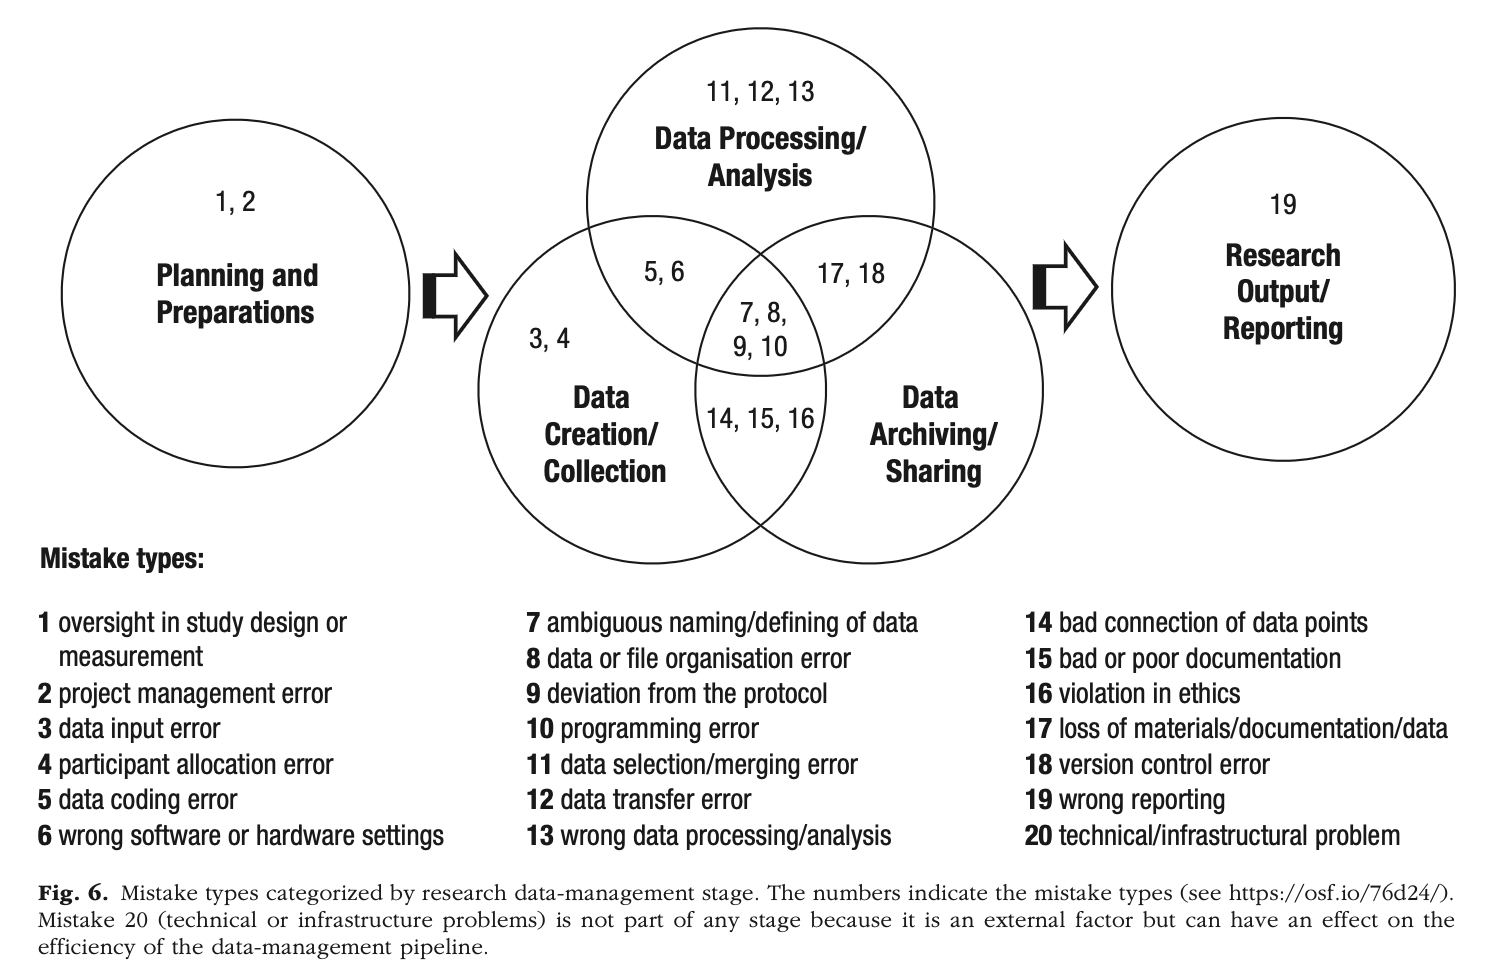
\includegraphics[width=0.9\linewidth]{./images/fallibility} 

}

\caption{Threats to the quality of the scientific process (Kovacs, Hoekstra, $\&$ Aczel, 2021)}\label{fig:fallibility}
\end{figure}

\hypertarget{open-data}{%
\section{Open Data}\label{open-data}}

\href{https://www.ukrn.org/2021/09/24/new-animated-explainer-on-data-sharing-now-available-to-view-online/}{Data sharing} is a core element in Open Science to enhance the credibility and trust on our research practices. Data sharing allows for the reproducibility of previous findings, while enabling others to inspect and spot mistakes in the data, the meta-data, or the research workflow. Additionally, it prevents---to a certain extent---the emergence of scientific fraud due to fabricated data/results/visualizations or to the use of questionable data analytical practices.

Data sharing also favors a swift progress in fields of research with difficulties in gaining access to relevant data (Gewin, 2016). It also enables researchers working at institutions based on countries with less resources and limited access to paywall journals and repositories.

However, sharing data has its drawbacks. Some researchers invest years to collect data that is very difficult to obtain (e.g., long-term primate behavior in Kibale National Park, Uganda) with the idea of completing a research project that will produce several outputs. If the data is shared in the first publication, sharing might be a problem for future publications (Hunt, 2019). To partially mitigate this problem, many journals allow researchers to publish the data sets in specialized data journals such as \href{https://www.nature.com/sdata/}{\emph{Nature}---\emph{Scientific Data}}, \href{https://academic.oup.com/gigascience/pages/About}{\emph{GigaScience}}, \href{https://bmcresnotes.biomedcentral.com}{\emph{BMC Research Notes}}, or \href{https://www.journals.elsevier.com/data-in-brief}{\emph{Data in brief}}. For example, in \emph{Nature}---\emph{Scientific Data}, these data descriptors are curated and can be modified to incorporate new data collected later. Moreover, Nature-titled journals do not consider prior Data Descriptor publications to compromise the novelty of new manuscript submissions if those manuscripts go substantially beyond a descriptive analysis of the data, and report important new scientific findings appropriate for the journal in question (Nature---Scientific Data, 2023).

Similarly, sharing data is not as easy and straightforward as it seems (e.g., to upload my anonymized csv file into a public repository). Researchers---especially postgraduate students and early career researchers-\/---must learn a new set of skills in order to publish their research products:

\begin{itemize}
\tightlist
\item
  Data curation
\item
  Data management plan
\item
  Storing, saving, archiving, and data preservation
\item
  Meta-data
\item
  Data analysis and visualization
\item
  Data wrangling
\item
  Reproducibility and data reuse
\item
  Compliance with FAIR data principles
\end{itemize}

\hypertarget{fair-data}{%
\section{FAIR Data}\label{fair-data}}

In 2016, the data journal \emph{Nature}---\emph{Scientific Data} published the \emph{FAIR Guiding Principles for Scientific Data Management and Stewardship} to clarify and guide researchers with the FAIR principles: Findable, Accessible, Interoperable, Reusable. The FAIR principles pivot around the idea of a continuum of ``machine-actionability'' in which machines can act autonomously on data objects, (1) in relation to the contextual metadata surrounding a digital object (\emph{what is it?}), and (2) when referring to the content (\emph{how do I process it/integrate it?}) (Wilkinson, 2016).

\begin{table}

\caption{\label{tab:Table13b}The FAIR Guiding Principles}
\centering
\resizebox{\linewidth}{!}{
\fontsize{14}{16}\selectfont
\begin{tabular}[t]{ll}
\toprule
\cellcolor[HTML]{EFEFEF}{Principles} & \cellcolor[HTML]{EFEFEF}{Guidelines}\\
\midrule
\cellcolor[HTML]{E1FAFF}{Findable} & \cellcolor[HTML]{E1FAFF}{F1. (meta)data are assigned a globally unique and persistent identifier}\\
\cellcolor[HTML]{E1FAFF}{} & \cellcolor[HTML]{E1FAFF}{F2. data are described with rich metadata (defined by R1 below)}\\
\cellcolor[HTML]{E1FAFF}{} & \cellcolor[HTML]{E1FAFF}{F3. metadata clearly and explicitly include the identifier of the data it describes}\\
\cellcolor[HTML]{E1FAFF}{} & \cellcolor[HTML]{E1FAFF}{F4. (meta)data are registered or indexed in a searchable resource}\\
\cellcolor[HTML]{D1FFEC}{Accessible} & \cellcolor[HTML]{D1FFEC}{A1. (meta)data are retrievable by their identifier using a standardized communications protocol}\\
\hspace{1em}\cellcolor[HTML]{D1FFEC}{} & \hspace{1em}\cellcolor[HTML]{D1FFEC}{A1.1 the protocol is open, free, and universally implementable}\\
\hspace{1em}\cellcolor[HTML]{D1FFEC}{} & \hspace{1em}\cellcolor[HTML]{D1FFEC}{A1.2 the protocol allows for an authentication and authorization procedure, where necessary}\\
\cellcolor[HTML]{D1FFEC}{} & \cellcolor[HTML]{D1FFEC}{A2. metadata are accessible, even when the data are no longer available}\\
\cellcolor[HTML]{FFF4D1}{Interoperable} & \cellcolor[HTML]{FFF4D1}{I1. (meta)data use a formal, accessible, shared, and broadly applicable language for knowledge representation}\\
\cellcolor[HTML]{FFF4D1}{} & \cellcolor[HTML]{FFF4D1}{I2. (meta)data use vocabularies that follow FAIR principles}\\
\cellcolor[HTML]{FFF4D1}{} & \cellcolor[HTML]{FFF4D1}{I3. (meta)data include qualified references to other (meta)data}\\
\cellcolor[HTML]{FFDBDB}{Reusable} & \cellcolor[HTML]{FFDBDB}{R1. meta(data) are richly described with a plurality of accurate and relevant attributes}\\
\hspace{1em}\cellcolor[HTML]{FFDBDB}{} & \hspace{1em}\cellcolor[HTML]{FFDBDB}{R1.1. (meta)data are released with a clear and accessible data usage license}\\
\hspace{1em}\cellcolor[HTML]{FFDBDB}{} & \hspace{1em}\cellcolor[HTML]{FFDBDB}{R1.2. (meta)data are associated with detailed provenance}\\
\hspace{1em}\cellcolor[HTML]{FFDBDB}{} & \hspace{1em}\cellcolor[HTML]{FFDBDB}{R1.3. (meta)data meet domain-relevant community standards}\\
\bottomrule
\end{tabular}}
\end{table}

\hypertarget{contributorship-credit}{%
\section{Contributorship (CRediT)}\label{contributorship-credit}}

\href{https://credit.niso.org}{The \emph{Contributor Roles Taxonomy}} (CRediT) has been designed to cover 14 key roles representing the spectrum of activities involved in the production of research outputs. Most of the big publishers (e.g., \href{https://www.nature.com/nature-portfolio/editorial-policies/authorship}{Nature}, \href{https://www.elsevier.com/authors/policies-and-guidelines/credit-author-statement}{Elsevier}, \href{https://uk.sagepub.com/en-gb/eur/credit}{SAGE}, \href{https://www.cell.com/pb/assets/raw/shared/guidelines/CRediT-taxonomy.pdf}{Cell Press}, \href{https://authorservices.wiley.com/author-resources/Journal-Authors/open-access/credit.html}{Wiley}) and psychological societies (\href{https://www.apa.org/pubs/journals/resources/publishing-tips/giving-credit}{American Psychological Association} {[}APA{]}), \href{https://www.psychologicalscience.org/observer/fully-credited-making-publishing-more-equitable}{Association for Psychological Science} {[}APS{]}) have made the CRediT system compulsory.

\textbf{The Contributor Roles Taxonomy (CRediT)}

Conceptualization

Data curation

Formal analysis

Funding acquisition

Investigation

Methodology

Project administration

Resources

Software

Supervision

Validation

Visualization

Writing---original draft

Writing---review and editing

Some of the desired consequences of this contributor system are to avoid:

\begin{itemize}
\item
  \textbf{Ghost authorship}: Authors who contributed to the work but are not listed, generally to hide a conflict of interest from editors, reviewers, and readers.
\item
  \textbf{Gift authorship}: Individuals given authorship credit who have not contributed in any substantive way to the research but are added to the author list by virtue of their stature in the organization.
\item
  \textbf{Orphan authorship}: Authors who contributed materially to the work but are omitted from the author list unfairly by the drafting team.
\item
  \textbf{Forged authorship}: Unwitting authors who had no part in the work but whose names are appended to the paper without their knowledge to increase the likelihood of publication.
\end{itemize}

\newpage

\hypertarget{references}{%
\section{References}\label{references}}

Arslan, R. C. (2019). \href{https://journals.sagepub.com/doi/10.1177/2515245919838783}{How to automatically document data with the codebook package to facilitate data reuse.} \emph{Advances in Methods and Practices in Psychological Science}, \emph{2}(2), 169---187.

European Commission. (2021). \href{https://research-and-innovation.ec.europa.eu/system/files/2019-12/ec_rtd_factsheet-open-science_2019.pdf}{Open Science} {[}Fact sheet{]}. European Union.

Gewin, V. (2016). \href{https://doi.org/10.1038/nj7584-117a}{Data sharing: An open mind on open data.} \emph{Nature}, \emph{529}, 117---119.

Hunt, L. T. (2019). \href{https://doi.org/10.1038/s41562-019-0560-3}{The life-changing magic of sharing your data.} \emph{Nature Human Behavior}, \emph{3}, 312---315.

John, L. K., Loewenstein, G., \& Prelec, D. (2012). \href{https://www.cmu.edu/dietrich/sds/docs/loewenstein/MeasPrevalQuestTruthTelling.pdf}{Measuring the prevalence of questionable research practices with incentives for truth telling.} \emph{Psychological Science}, \emph{23}(5), 524---532.

Klein O., Hardwicke T. E., Aust F., Breuer J., Danielsson H., Mohr A. H., Ijzerman H., Nilsonne G., Vanpaemel W., Frank M. C. (2018). \href{https://online.ucpress.edu/collabra/article/4/1/20/112998/A-Practical-Guide-for-Transparency-in}{A practical guide for transparency in psychological science.} \emph{Collabra: Psychology}, \emph{4}(1):20.

Kovacs, M., Hoekstra, R., \& Aczel, B. (2021). \href{https://journals.sagepub.com/doi/full/10.1177/25152459211045930}{The role of human fallibility in psychological research: A survey of mistakes in data management.} \emph{Advances in Methods and Practices in Psychological Science}, \emph{4}(4), 1---13.

Miedema, F. (2022). \href{https://library.oapen.org/handle/20.500.12657/51498}{Open Science: The very idea.} Springer.

Nature--Scientific Data (2023). \href{https://www.nature.com/sdata/faq}{Frequently Asked Questions.} Retrieved from Nature--Scientific Data website: \url{https://www.nature.com/sdata/faq}

Open Science Collaboration. (2015). \href{https://www.science.org/doi/10.1126/science.aac4716}{Estimating the reproducibility of psychological science.} \emph{Science}, \emph{349}(6251), 1---8.

Spellman, B., Gilbert, E. A., \& Corker, K. S. (2017, September 20). \href{https://psyarxiv.com/ak6jr/}{Open Science: What, Why, and How.} \url{https://psyarxiv.com/ak6jr/}

UK Reproducibility Network. (2021, September). \href{https://bpb-eu-w2.wpmucdn.com/blogs.bristol.ac.uk/dist/b/631/files/2021/09/UKRN-ToR-v3.3.pdf}{Terms of Reference.} Version 3.3.

United Nations Educational, Scientific, and Cultural Organization. (2021, November). \href{https://www.unesco.org/en/open-science}{UNESCO Recommendation on Open Science} (Programme Document SC-PCB-SPP/2021/OS/UROS). Retrieved from the United Nations Educational, Scientific, and Cultural Organization website: \url{https://unesdoc.unesco.org/ark:/48223/pf0000379949}

Wilkinson, M. D., Dumontier, M., Aalbersberg, I. J., Appleton, G., Axton, M., Baak, A., Blomberg, N., Boiten, J. W., da Silva Santos, L. B., Bourne, P. E., Bouwman, J., Brookes, A. J., Clark, T., Crosas, M., Dillo, I., Dumon, O., Edmunds, S., Evelo, C. T., Finkers, R., Gonzalez-Beltran, A., \ldots{} Mons, B. (2016). \href{https://www.nature.com/articles/sdata201618}{The FAIR Guiding Principles for scientific data management and stewardship.} \emph{Scientific Data}, \emph{3}:160018.

\hypertarget{introduction-to-r}{%
\chapter{Introduction to R}\label{introduction-to-r}}

\begin{quote}
\textbf{LEARNING OUTCOMES}

\begin{itemize}
\tightlist
\item
  Identify the capabilities of R and RStudio's environment and appraise their functionality.
\item
  Distinguish between R functions, objects, and diverse data wrangling approaches.
\item
  Apply basic programming skills to import and organize the data using classic data wrangling approaches and the \textbf{tidyverse} grammar.
\item
  Evaluate the R code and appraise the outputs to demonstrate a satisfactory level of basic programming skills in R.
\end{itemize}
\end{quote}

\textbf{R} is a programming language and an open-source software environment for statistical computing and graphics available for Windows, MacOS, and Linux operating systems (R Core Team, 2023). R is an interactive environment for data science that enables us to import, manipulate, model, and visualize data to effectively communicate our results (Wickham \& Grolemund, 2017). The use of R also promotes transparency and open research, with a clear focus on supporting reproducibility policies (Gandrud, 2015).

R, in its most basic form, is composed by (1) a \emph{script} in which we write the lines of R code that we run, and (2) the \emph{console} that displays the results and debugging (Figure 2.1). If we generate a plot, it will emerge as a pop-up window, showing one plot at a time. For more details on what is R, click \href{http://www.r-project.org}{here}.

\begin{figure}

{\centering 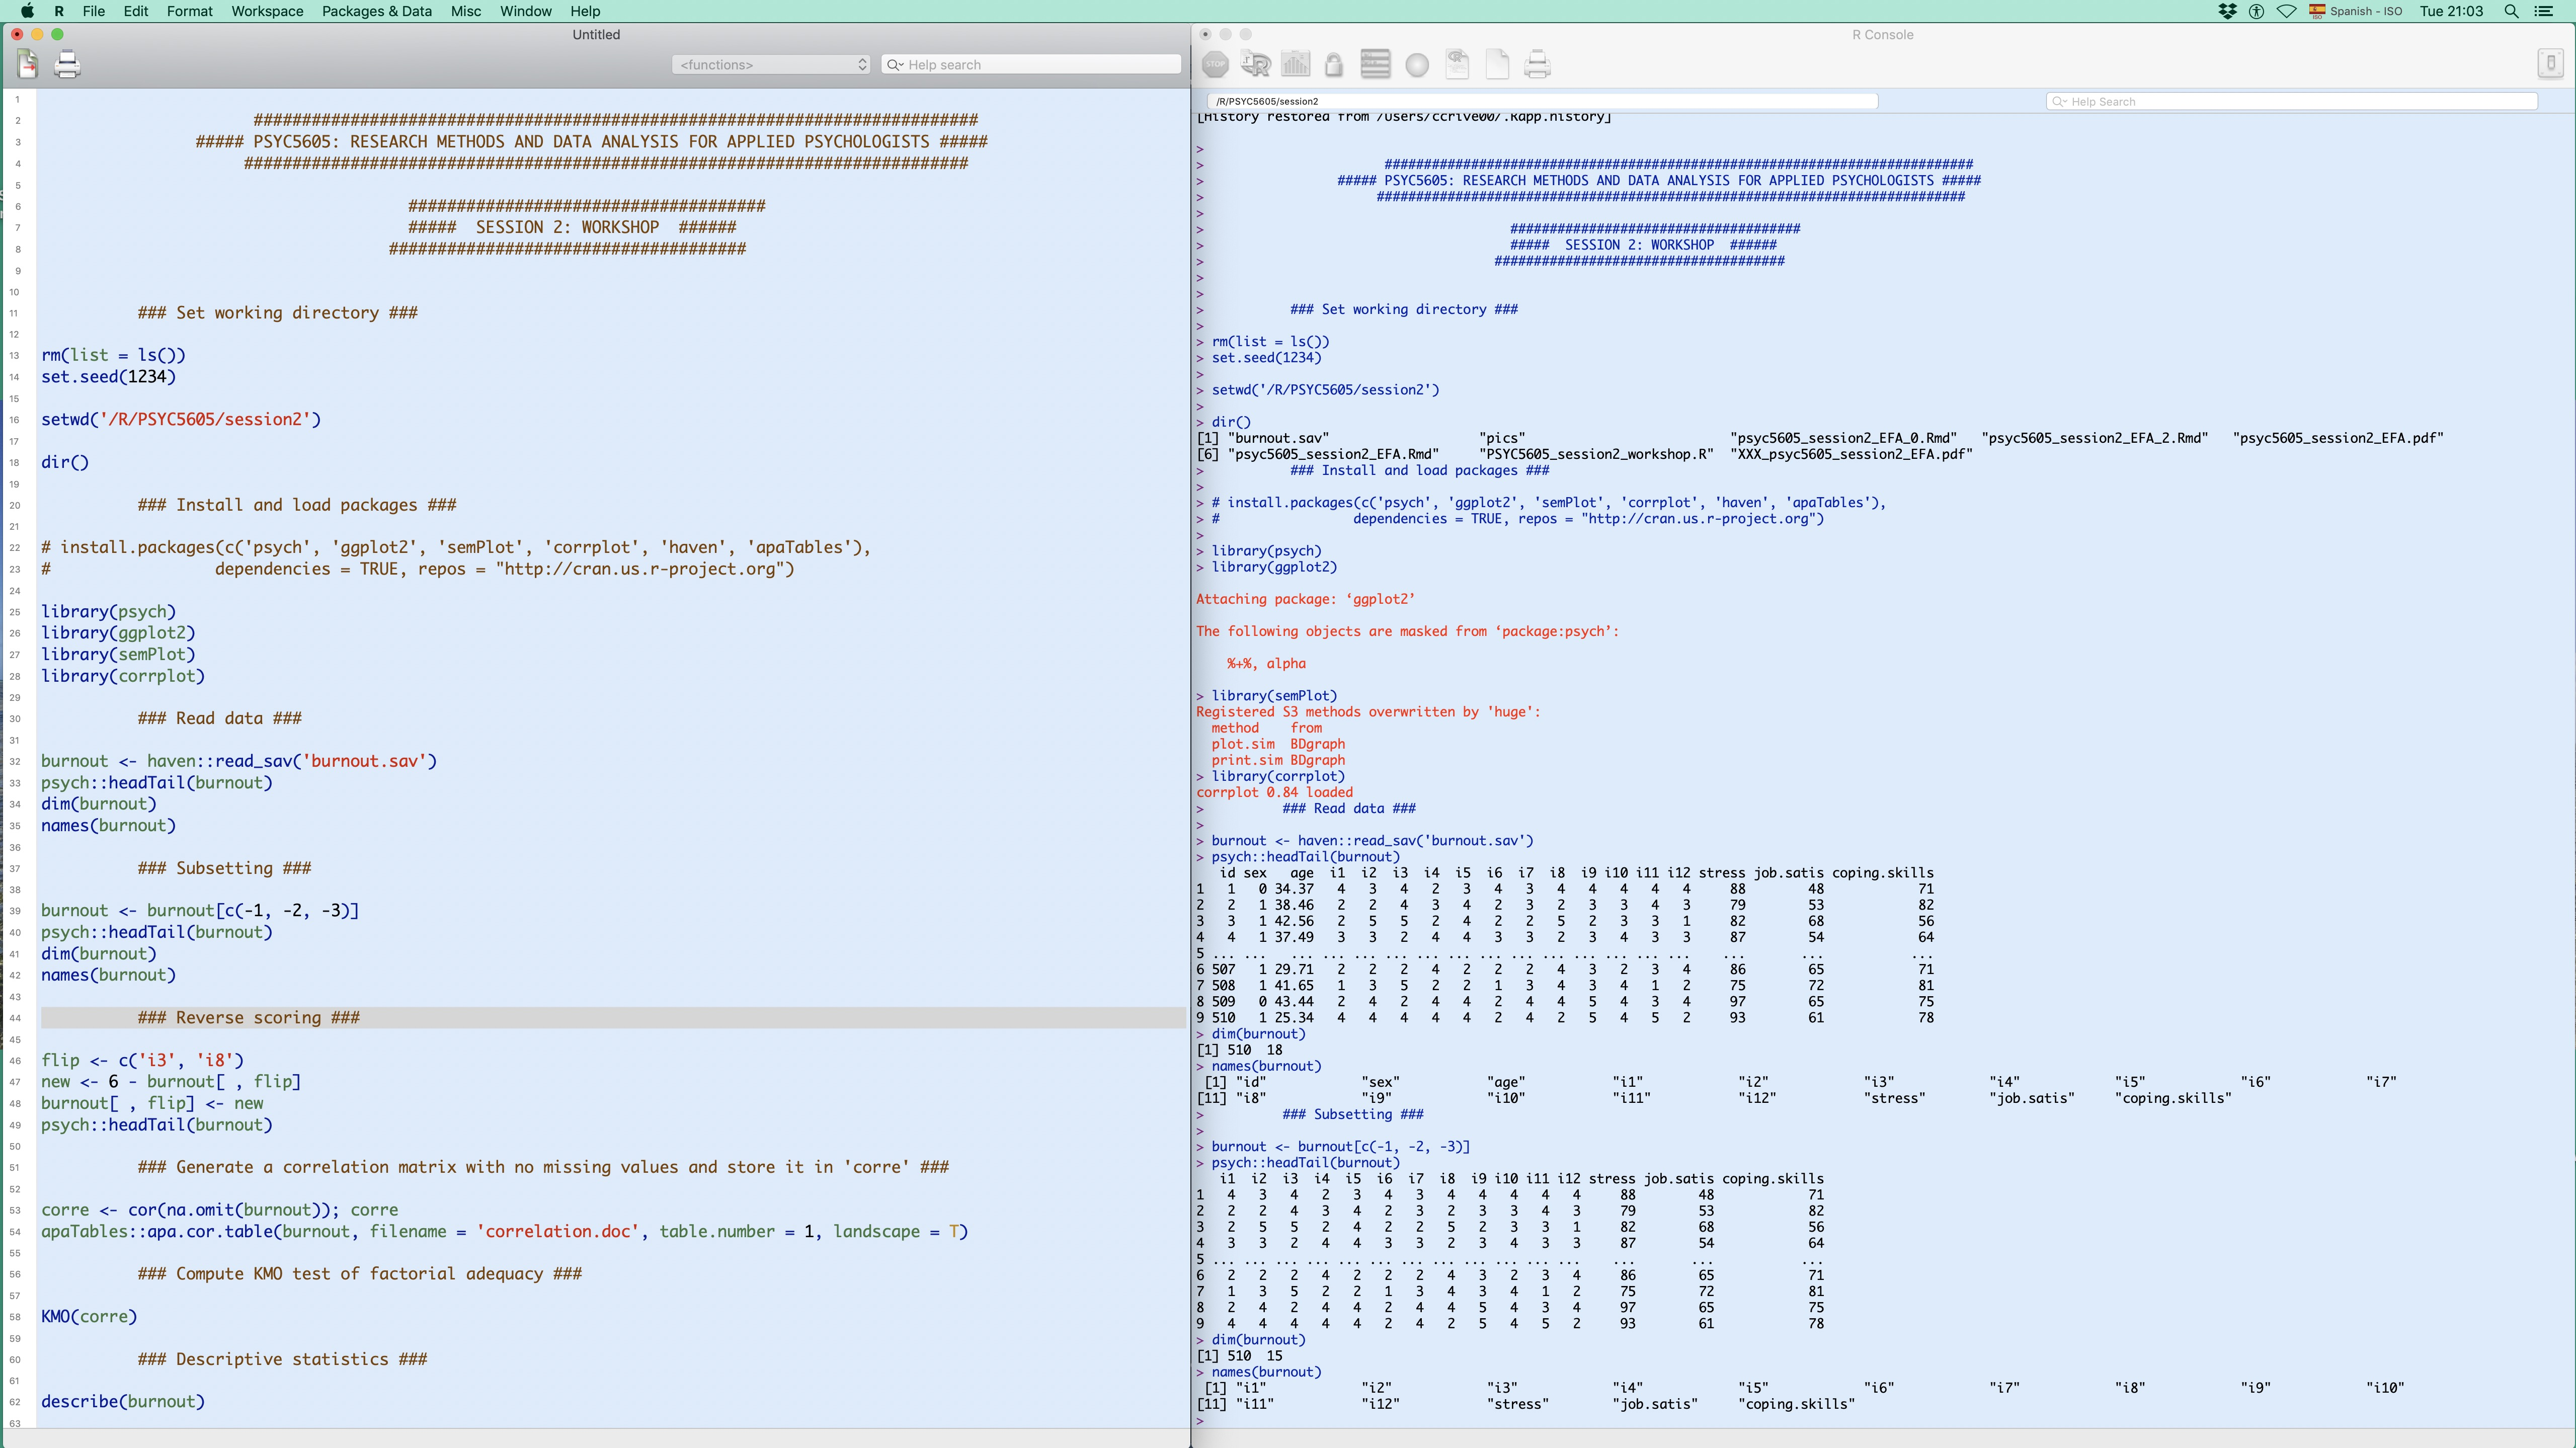
\includegraphics[width=1\linewidth]{./images/R_panels} 

}

\caption{R displayed in two panels: Script (left) and Console (right).}\label{fig:Rpanels}
\end{figure}

\textbf{Why Use R?}

It is a free and open-access programming environment for data science

Reproducible and transparent research in psychological science

Unlimited capabilities for data science (e.g., analysis, modelling, visualization)

It is dynamic. R is constantly evolving. It provides state-of-the-art solutions for any imaginable field (e.g., economics, psychology, genetics, medicine, ecology, sociology, computational physics, geography, psychometrics)

R has the biggest global community providing all sorts of free resources to support learners (e.g., \href{https://cran.r-project.org/doc/manuals/r-release/R-intro.html}{reference manuals}, \href{https://bookdown.org}{books}, \href{http://milton-the-cat.rocks/learnr/r/r_getting_started/\#section-installing-r-and-rstudio}{on-line tutorials}, \href{https://debruine.github.io/lmem_sim/}{R code and notebooks}, \href{https://github.com/rstudio/cheatsheets/blob/main/base-r.pdf}{cheat sheets}, \href{https://community.rstudio.com}{Internet forums})

R is more efficient than any other commercial software

UK universities teaching 21st century data science with R: \href{https://psyteachr.github.io}{University of Glasgow}, Lancaster University, \href{https://www.ntu.ac.uk/about-us/events/events/2022/6/teaching-statistics-with-r-in-psychology}{Nottingham Trent University}, \href{https://bookdown.org/animestina/dapr1_labs/}{University of Edinburgh}, University of Lincoln, University of Manchester, University of Plymouth, University of Sussex, Queen Mary University of London, University of Sheffield, University of Essex, Oxford University, King's College, University of Warwick\ldots{}

Employability

\hypertarget{what-is-rstudio}{%
\section{What is RStudio?}\label{what-is-rstudio}}

\textbf{RStudio} is an Integrated Development Environment (IDE) for R. RStudio facilitates the task of coding by providing an enhanced programming experience. First, RStudio is free and easy to learn. Second, RStudio's elements are displayed in a four-panel display: the \emph{code editor} (the script), the \emph{console} (the results and debugging), the \emph{global environment} (e.g., R objects, history of our session), and a \emph{notebook} that includes different active tabs (e.g., plots, packages, help) (Figure 2.2). Last, there is an optimal integration of the different panels and tabs to run R sessions and projects smoothly.

\begin{figure}

{\centering 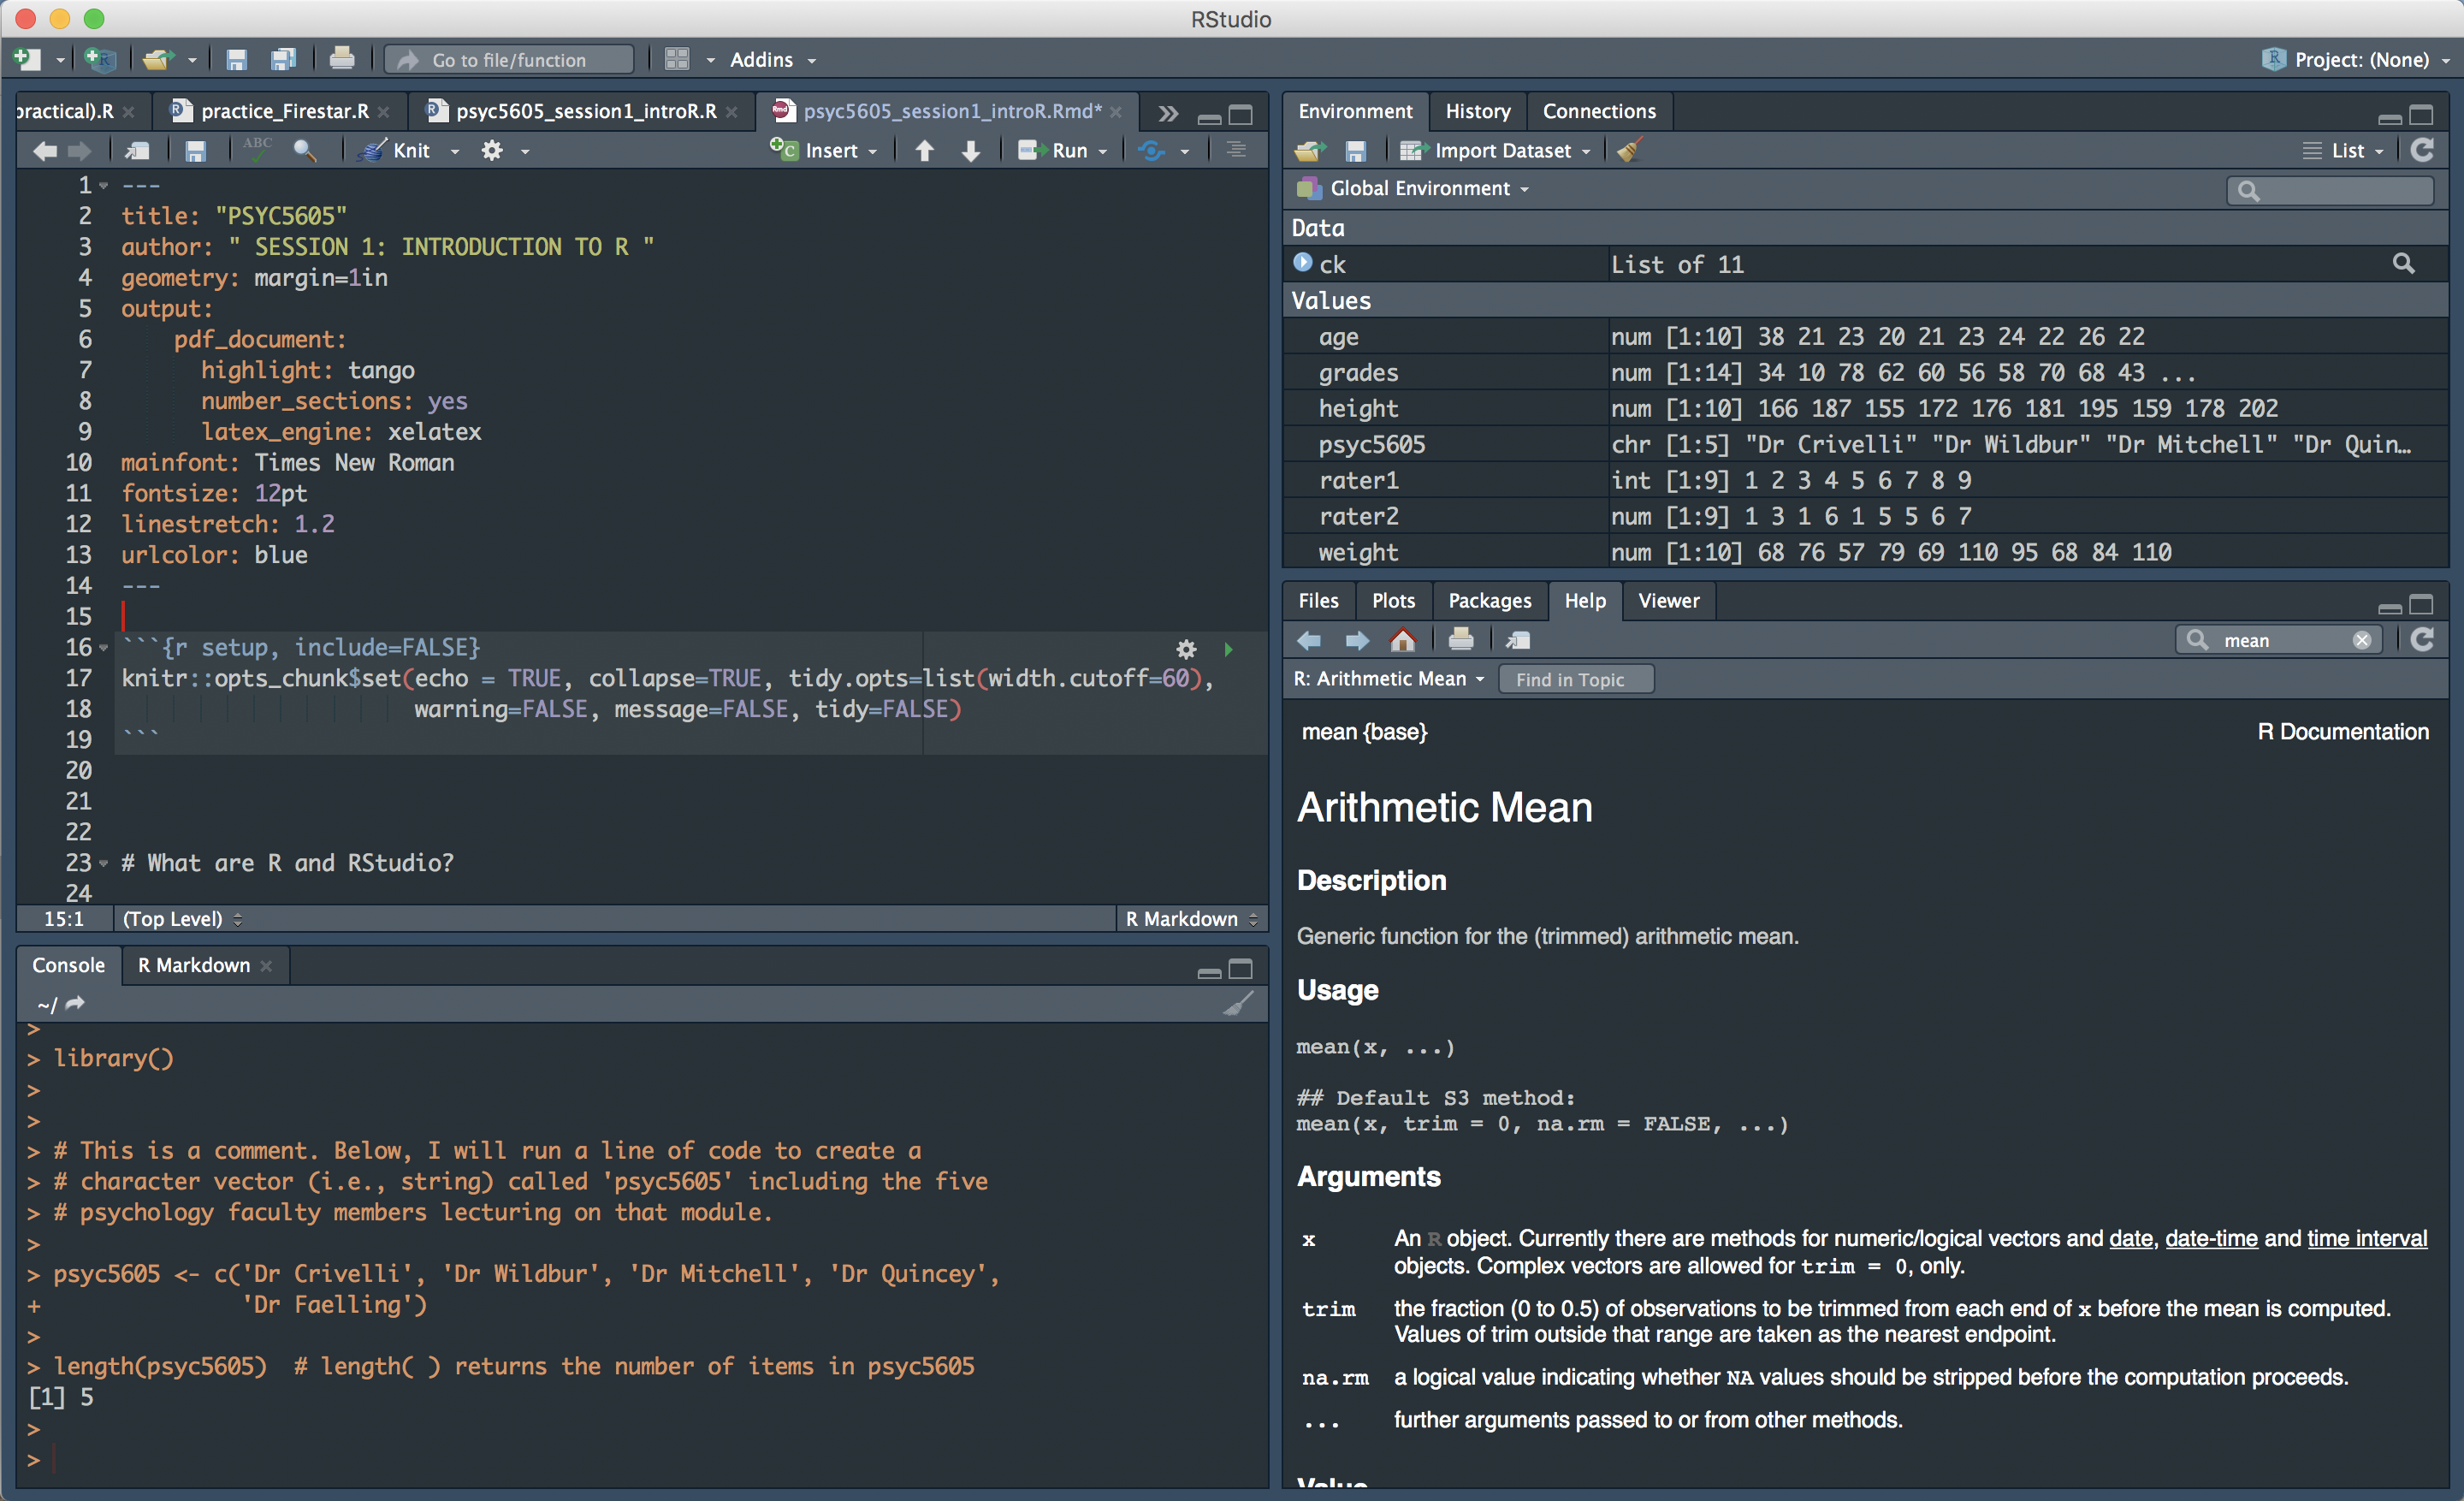
\includegraphics[width=1\linewidth]{./images/RStudio_panels} 

}

\caption{RStudio's four-panel display.}\label{fig:RStudio}
\end{figure}

\textbf{Why Use RStudio?}

RStudio's main components are integrated into a four-pane layout: the \emph{code editor} (the script), the \emph{console} (the results and debugging), the \emph{global environment} (the R objects, history of our session), and a \emph{notebook} to hold tabs for the files/plots/packages/help/viewer

The code editor is feature-rich and integrated with the built-in console

The code editor and console are efficiently linked to the files/plots/packages/help/viewer panels

RStudio is available for Windows, MacOS, and Linux

RStudio is easy to learn

For more details on what is RStudio, click \href{https://posit.co/products/open-source/rstudio/}{here}

\hypertarget{lets-get-started}{%
\section{Let's get started!}\label{lets-get-started}}

\hypertarget{running-a-line-of-code}{%
\subsection{Running a line of code}\label{running-a-line-of-code}}

There are several ways to run a line of code:

\begin{itemize}
\item
  Highlight the line of code and click on the button \textbf{Run} (\(\Rightarrow\) \texttt{Run}) displayed on the upper right side of the \emph{code editor}.
\item
  Highlight the line of code that you want to run and press \textbf{Ctrl + Enter} (Windows) or \textbf{Cmd + Enter} (MacOS).
\item
  Place the cursor on the line of code and click on the button \textbf{Run} (\(\Rightarrow\) \texttt{Run}).
\item
  Press \textbf{Ctrl + Shift + S} (Windows) or \textbf{Cmd + Shift + S} (MacOS) to run the code of an entire script.
\item
  Type a line of code directly into the \emph{console} or copy a line of code from the \emph{code editor} and paste it into the \emph{console} after the prompt (\texttt{\textgreater{}}). Then, press \textbf{Enter} on the \emph{console}.
\end{itemize}

\hypertarget{adding-comments-on-r-scripts}{%
\subsection{Adding comments on R scripts}\label{adding-comments-on-r-scripts}}

It is useful to add comments before chunks of R code to organize the session and to inform others that might be interested in reproducing our session and evaluating our outputs. The hash mark (\texttt{\#}) is used to make comments by placing the symbol at the beginning of a line of code. R won't execute the line of code that is preceded by one or more hash mark symbols.

\begin{Shaded}
\begin{Highlighting}[]

\CommentTok{\# This is a comment}
\CommentTok{\# Raise 5 to the power of 2}

\DecValTok{5} \SpecialCharTok{\^{}} \DecValTok{2}
\DocumentationTok{\#\# [1] 25}

\FunctionTok{sqrt}\NormalTok{(}\DecValTok{25}\NormalTok{)  }\CommentTok{\# sqrt(x) returns the square root of x}
\DocumentationTok{\#\# [1] 5}
\end{Highlighting}
\end{Shaded}

\hypertarget{starting-a-session-in-rstudio}{%
\section{Starting a session in RStudio}\label{starting-a-session-in-rstudio}}

\hypertarget{setting-the-global-options}{%
\subsection{Setting the global options}\label{setting-the-global-options}}

It is possible to customize RStudio (e.g., code, appearance, organization of panels) to adapt it to our needs and preferences. To do so, click on the main \textbf{RStudio menu bar} \(\rightarrow\) \textbf{Tools} \(\rightarrow\) \textbf{Global Options}. Although there are many available options to customize RStudio sessions, we will mention below some of the most interesting features to inspect in the \emph{global options} settings:

\begin{itemize}
\item
  \textbf{General}: It is convenient to start a new R session to avoid carrying over variable corruptions. Consequently, do not restore or save .RData files into the workspace at startup.
\item
  \textbf{Code-Display options}: To enhance the usability experience, enable \emph{soft-wrap R source files}, \emph{highlight selected word}, \emph{show line numbers}, and \emph{blinking cursor}. In the option \emph{show margin}, set the margin column to 60.
\item
  \textbf{Appearance}: The customization of the \emph{editor} and \emph{console}'s appearance (e.g., font size) is pivotal as we will spend a lot of time looking at the computer screen when programming. For example, the use of dark background colors (e.g., material, chrome) is very popular among programmers because it minimizes eye strain or fatigue. If you are a low vision user, the high contrast generated by a dark background and white text will be beneficial as well.
\item
  \textbf{Pane Layout}: It is possible to reorganize the location of the panels. Likewise, it is possible to show or hide the different tabs available in the \emph{global environment} and \emph{notebook}. For instance, we could arrange the \emph{source} on the upper left-hand side, inspecting the output of the code that we run underneath or on the right hand side (the \emph{console} would be located on the bottom left corner or on the upper right corner respectively).
\end{itemize}

\hypertarget{first-lines-of-code}{%
\subsection{First lines of code}\label{first-lines-of-code}}

Every session will start with three lines of code that we will include at the beginning of our R script. First, we will use the function \texttt{rm()} (i.e., remove) to delete any R object stored in the \emph{global environment}. We want to start each session anew, without carrying over R objects from previous sessions. Second, we will set the randomization seed with the function \texttt{set.seed()} to reproduce the R objects and outputs of any simulated data and computation. Last, we will turn off the scientific notation used in R.

\begin{Shaded}
\begin{Highlighting}[]

\FunctionTok{rm}\NormalTok{(}\AttributeTok{list =} \FunctionTok{ls}\NormalTok{())}
\FunctionTok{set.seed}\NormalTok{(}\DecValTok{1234}\NormalTok{)  }
\FunctionTok{options}\NormalTok{(}\AttributeTok{scipen=}\DecValTok{999}\NormalTok{)}
\end{Highlighting}
\end{Shaded}

\hypertarget{setting-the-working-directory}{%
\subsection{Setting the working directory}\label{setting-the-working-directory}}

There is a point-and-click approach to set the working directory for each R session. To do so, click on the main \textbf{RStudio menu bar} \(\rightarrow\) \textbf{Session} \(\rightarrow\) \textbf{Set Working Directory} \(\rightarrow\) \textbf{Choose Directory}. Then, select the desired folder to store all the files of the session (e.g., the R file with the code, data sets).

When exporting plots and files, these files will be saved and stored locally in the working directory already set at the beginning of the session. For example, we created a folder called \emph{R} located in the main SSD MacOS/C: hard drive that includes the directories of all our R projects. At a lower level, we created another folder called \emph{psyc3012} (Data Science with R) to store the current R project that, in turn, includes one folder per session (e.g., \emph{session1}, \emph{session2}, \emph{session3}).

\textbf{Setting the path for the working directory}

The path should be short

Create a folder called \emph{R} in your PC (C:) or MacOS (HD/SSD) hard drives. Then, create folders for different projects in the \emph{R} folder

Use short names with no spaces (e.g., do not use a folder name such as \emph{session 1}, but \emph{session1} or \emph{session\_1})

R is case sensitive (\emph{psyc3012} differs from \emph{PSYC3012})

Use single (`\emph{x}') or double quotes (``\emph{x}'') because the path is a character string

The function \texttt{getwd()} finds the path to the folder of our current working directory, whereas the function \texttt{setwd()} sets the working directory's path.

\begin{Shaded}
\begin{Highlighting}[]

\FunctionTok{getwd}\NormalTok{()}
\FunctionTok{setwd}\NormalTok{(}\StringTok{\textquotesingle{}\textasciitilde{}/R/psyc3012/session1\textquotesingle{}}\NormalTok{)}
\end{Highlighting}
\end{Shaded}

\hypertarget{r-objects-and-functions}{%
\section{R objects and functions}\label{r-objects-and-functions}}

There are different kinds of entities that we identify as objects. Here, we will distinguish between R objects of different data structures (e.g., matrices, vectors, data frames, lists) and ``recursive'' objects such as those of mode \emph{function} (Lander, 2017; Venables et al., 2009). We will refer to the latter as functions and to the former as R objects. In sum, we will use functions (e.g., \texttt{mean()}, \texttt{boxplot()}) to execute commands on R objects (e.g., atomic vectors, data frames, matrices).

\hypertarget{functions}{%
\subsection{Functions}\label{functions}}

Let's imagine that we would like to command a robot to do something for us. We simply need to learn the robot's language (i.e., rules of grammar, syntax, vocabulary, code), so it can decode our commands and execute our orders. Any programming language will work in a similar way. For instance, we will need to read data from files (e.g., text file, CSV file, SPSS file) or to simulate our own data. These data should be appropriately stored and saved into R's \emph{global environment} to be able to manipulate and organize our data (e.g., merge, subset, select, rename), to model and visualize the data, and to publish the results. To complete those tasks, we must use appropriate functions on data structures of the same mode.

\hypertarget{the-c-function}{%
\subsubsection{\texorpdfstring{The \texttt{c()} function}{The c() function}}\label{the-c-function}}

The \texttt{c()} function is usually referred as the concatenate or combine function. It combines two or more elements of the same mode (e.g., numerical values, character strings, logical values) to create vectors.

\begin{Shaded}
\begin{Highlighting}[]

\FunctionTok{c}\NormalTok{(}\DecValTok{16}\NormalTok{, }\DecValTok{71}\NormalTok{, }\DecValTok{172}\NormalTok{, }\DecValTok{53}\NormalTok{, }\DecValTok{77}\NormalTok{)}
\DocumentationTok{\#\# [1]  16  71 172  53  77}

\FunctionTok{c}\NormalTok{(}\StringTok{\textquotesingle{}Hylobates\textquotesingle{}}\NormalTok{, }\StringTok{\textquotesingle{}Pongo\textquotesingle{}}\NormalTok{, }\StringTok{\textquotesingle{}Gorilla\textquotesingle{}}\NormalTok{, }\StringTok{\textquotesingle{}Pan\textquotesingle{}}\NormalTok{, }\StringTok{\textquotesingle{}Homo\textquotesingle{}}\NormalTok{)}
\DocumentationTok{\#\# [1] "Hylobates" "Pongo"     "Gorilla"   "Pan"       "Homo"}

\FunctionTok{c}\NormalTok{(}\ConstantTok{FALSE}\NormalTok{, }\ConstantTok{TRUE}\NormalTok{, }\ConstantTok{TRUE}\NormalTok{, }\ConstantTok{TRUE}\NormalTok{, }\ConstantTok{TRUE}\NormalTok{)}
\DocumentationTok{\#\# [1] FALSE  TRUE  TRUE  TRUE  TRUE}
\end{Highlighting}
\end{Shaded}

\hypertarget{r-objects}{%
\subsection{R objects}\label{r-objects}}

R objects such as character strings and numeric vectors, data frames, matrices or lists are saved and stored in R's \emph{global environment} when we assign them to a name using the assignment operator (\texttt{name} \(\gets\) \texttt{data}). The \emph{console} shows the object only if it is recalled. To produce the assignment operator in Windows/Linux operating systems press \textbf{Alt} + \textbf{-}. Alternatively, press \textbf{Option} + \textbf{-} if using MacOS.

As a computing programming language, R executes our commands to produce certain outcomes. Sometimes those outcomes will appear on the \emph{console} (e.g., estimating the arithmetic mean on a numerical vector). Other times, however, these commands won't produce effects on the \emph{console}. For example, when we create a vector, it will only appear in the \emph{global environment} tab unless it will be recalled in the same line of code preceded by a semicolon (\texttt{;}) or plaxed on a line of code below.

\begin{Shaded}
\begin{Highlighting}[]

\NormalTok{weight }\OtherTok{\textless{}{-}} \FunctionTok{c}\NormalTok{(}\DecValTok{16}\NormalTok{, }\DecValTok{71}\NormalTok{, }\DecValTok{172}\NormalTok{, }\DecValTok{53}\NormalTok{, }\DecValTok{77}\NormalTok{); weight}
\DocumentationTok{\#\# [1]  16  71 172  53  77}

\NormalTok{apes }\OtherTok{\textless{}{-}} \FunctionTok{c}\NormalTok{(}\StringTok{\textquotesingle{}Hylobates\textquotesingle{}}\NormalTok{, }\StringTok{\textquotesingle{}Pongo\textquotesingle{}}\NormalTok{, }\StringTok{\textquotesingle{}Gorilla\textquotesingle{}}\NormalTok{, }\StringTok{\textquotesingle{}Pan\textquotesingle{}}\NormalTok{, }\StringTok{\textquotesingle{}Homo\textquotesingle{}}\NormalTok{)}
\NormalTok{apes}
\DocumentationTok{\#\# [1] "Hylobates" "Pongo"     "Gorilla"   "Pan"       "Homo"}
\end{Highlighting}
\end{Shaded}

If we don't assign a set of values to any given name to create an R object, these values won't be saved into the \emph{global environment}. Therefore, we won't be able to recall the object for future computations.

\begin{Shaded}
\begin{Highlighting}[]

\FunctionTok{c}\NormalTok{(}\DecValTok{16}\NormalTok{, }\DecValTok{71}\NormalTok{, }\DecValTok{172}\NormalTok{, }\DecValTok{53}\NormalTok{, }\DecValTok{77}\NormalTok{)}
\DocumentationTok{\#\# [1]  16  71 172  53  77}
\end{Highlighting}
\end{Shaded}

Instead of creating an R object first, we could be tempted to paste a vector into a function. This approach is not efficient---specially with large data structures---and it should be avoided. Given the outstanding possibilities that R offers, we should create R objects and use functions on them to model and visualize the data.

\begin{Shaded}
\begin{Highlighting}[]

\FunctionTok{mean}\NormalTok{(}\FunctionTok{c}\NormalTok{(}\DecValTok{16}\NormalTok{, }\DecValTok{71}\NormalTok{, }\DecValTok{172}\NormalTok{, }\DecValTok{53}\NormalTok{, }\DecValTok{77}\NormalTok{))}
\DocumentationTok{\#\# [1] 77.8}

\NormalTok{weight.apes }\OtherTok{\textless{}{-}} \FunctionTok{c}\NormalTok{(}\DecValTok{16}\NormalTok{, }\DecValTok{71}\NormalTok{, }\DecValTok{172}\NormalTok{, }\DecValTok{53}\NormalTok{, }\DecValTok{77}\NormalTok{)}

\FunctionTok{mean}\NormalTok{(weight.apes)}
\DocumentationTok{\#\# [1] 77.8}
\FunctionTok{mean}\NormalTok{(weight.apes, }\AttributeTok{trim =}\NormalTok{ .}\DecValTok{20}\NormalTok{)}
\DocumentationTok{\#\# [1] 67}
\FunctionTok{median}\NormalTok{(weight.apes)}
\DocumentationTok{\#\# [1] 71}
\FunctionTok{sd}\NormalTok{(weight.apes)}
\DocumentationTok{\#\# [1] 57.78148}
\FunctionTok{length}\NormalTok{(weight.apes)}
\DocumentationTok{\#\# [1] 5}

\FunctionTok{barplot}\NormalTok{(weight.apes, }\AttributeTok{ylab =} \StringTok{\textquotesingle{}Weight (Kg)\textquotesingle{}}\NormalTok{, }\AttributeTok{xlab =} \StringTok{\textquotesingle{}Apes\textquotesingle{}}\NormalTok{,}
        \AttributeTok{col =} \StringTok{\textquotesingle{}coral3\textquotesingle{}}\NormalTok{, }\AttributeTok{ylim =} \FunctionTok{c}\NormalTok{(}\DecValTok{0}\NormalTok{, }\DecValTok{200}\NormalTok{),}
        \AttributeTok{names.arg =} \FunctionTok{c}\NormalTok{(}\StringTok{\textquotesingle{}Hylobates\textquotesingle{}}\NormalTok{, }\StringTok{\textquotesingle{}Pongo\textquotesingle{}}\NormalTok{, }\StringTok{\textquotesingle{}Gorilla\textquotesingle{}}\NormalTok{, }\StringTok{\textquotesingle{}Pan\textquotesingle{}}\NormalTok{, }\StringTok{\textquotesingle{}Homo\textquotesingle{}}\NormalTok{))}
\end{Highlighting}
\end{Shaded}

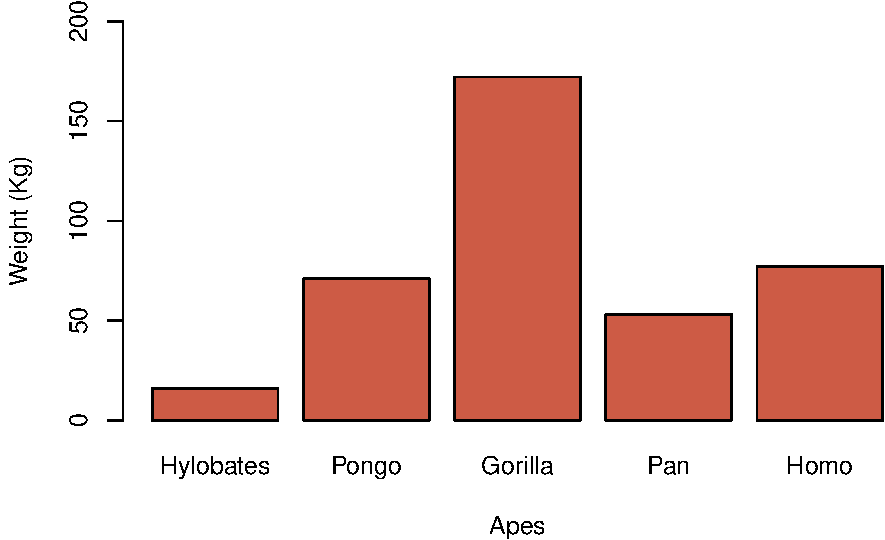
\includegraphics{_main_files/figure-latex/assignment_3-1.pdf}

\textbf{Naming objects}

R is case sensitive (e.g., the R object \emph{weight} differs from \emph{Weight})

Do not start with a number or special characters (e.g., +, -, \&, *, ?)

Using lower (e.g., \emph{weight.apes}, \emph{x}, \emph{m2spr34}) rather than an upper case letters (e.g., \emph{Weight.Apes}, \emph{X}, \emph{M2spr34}) facilitates the programming flow

Do not use names of functions to name R objects (e.g., \texttt{data()}, \texttt{mean()}, \texttt{plot()}, \texttt{factor()})

When using several words, do not leave spaces. Alternatively, use the full stop, underscore, or a combination of UPPER and lower case letters (e.g., \emph{g.spatial.males}, \emph{g\_fluid\_females}, \emph{gCrystallized})

Use short, but informative names (e.g., \emph{g.spatial.m}, \emph{g\_fluid\_f}, \emph{gCrystal})

\hypertarget{applying-functions-to-objects}{%
\subsection{Applying functions to objects}\label{applying-functions-to-objects}}

Functions work on data stored in R objects and saved in the \emph{global environment}. We will place the name of the R object within the parentheses of functions, executing the command of the function on R objects. Below, we will compute the arithmetic mean (\emph{M} = 52.1) and estimate the length (\emph{N} = 10) of one numeric vector named \emph{age}.

\begin{Shaded}
\begin{Highlighting}[]

\NormalTok{age }\OtherTok{\textless{}{-}} \FunctionTok{c}\NormalTok{(}\DecValTok{37}\NormalTok{, }\DecValTok{19}\NormalTok{, }\DecValTok{74}\NormalTok{, }\DecValTok{62}\NormalTok{, }\DecValTok{51}\NormalTok{, }\DecValTok{56}\NormalTok{, }\DecValTok{58}\NormalTok{, }\DecValTok{76}\NormalTok{, }\DecValTok{45}\NormalTok{, }\DecValTok{43}\NormalTok{)}
\FunctionTok{mean}\NormalTok{(age)}
\DocumentationTok{\#\# [1] 52.1}
\FunctionTok{length}\NormalTok{(age)}
\DocumentationTok{\#\# [1] 10}
\end{Highlighting}
\end{Shaded}

Functions usually include arguments that allow us to modify their default settings. For example, the function \texttt{mean()} computes the arithmetic mean on the R object placed within parentheses. In the previous example, some outliers (e.g., 19, 76) might be distorting the estimation of the \emph{age} distribution's central tendency. Luckily, the argument \texttt{trim} can be set from 0 (no trimming) to 0.5 (maximum trimming) to compute robust estimators of central tendency. By trimming 20\% of the observations from each tail of the distribution (\texttt{trim\ =\ .20}), we will compute 20\% trimmed means---a robust estimator of central tendency (Wilcox, 2016). The maximum trimming (\texttt{trim\ =\ .50}) computes the median as it only considers the central value of the distribution.

\begin{Shaded}
\begin{Highlighting}[]

\FunctionTok{mean}\NormalTok{(age, }\AttributeTok{trim =} \DecValTok{0}\NormalTok{)}
\DocumentationTok{\#\# [1] 52.1}
\FunctionTok{mean}\NormalTok{(age, }\AttributeTok{trim =}\NormalTok{ .}\DecValTok{20}\NormalTok{)}
\DocumentationTok{\#\# [1] 52.5}
\FunctionTok{mean}\NormalTok{(age, }\AttributeTok{trim =}\NormalTok{ .}\DecValTok{50}\NormalTok{)}
\DocumentationTok{\#\# [1] 53.5}
\FunctionTok{median}\NormalTok{(age)}
\DocumentationTok{\#\# [1] 53.5}
\end{Highlighting}
\end{Shaded}

\hypertarget{getting-help}{%
\subsection{Getting help}\label{getting-help}}

All R functions are included in packages that are created and maintained by their authors (e.g., statisticians, psychologists, biologists, sociologists). R packages are freely available on the Internet at the \href{https://cran.r-project.org/web/packages/}{\emph{Comprehensive R Archive Network}} or CRAN. Every package has its own documentation that describes and explains how to use the functions of each package. We can also access to cheat sheets, on-line learning tools, forums and on-line communities, blogs, or even open-access books created in R using \href{https://bookdown.org/yihui/bookdown/}{\textbf{bookdown}} (Xie, 2017; Xie, Allaire, \& Grolemund, 2019).

RStudio includes the documentation of functions and packages in the \emph{Help} tab. For example, if we search for the function \texttt{mean()}, we will find the documentation for this function included in R's package \textbf{base}. Another way to access to the documentation of packages and functions when help is required is to use the function \texttt{help()} or the question mark (\texttt{?}) followed by the name of the function.

\begin{Shaded}
\begin{Highlighting}[]

\FunctionTok{help}\NormalTok{(mean)}
\NormalTok{?mean}
\end{Highlighting}
\end{Shaded}

\hypertarget{packages}{%
\section{Packages}\label{packages}}

A package is a collection of functions, data sets, and compiled R code for a given purpose (e.g., visualize data, perform specific data analytical techniques). First, we must install the packages on our computer. These packages will be downloaded and stored locally just once. Then, we will upload these packages into our R session when required. The function \texttt{.libPaths()} shows the directory in which our packages are installed.

\begin{Shaded}
\begin{Highlighting}[]

\FunctionTok{.libPaths}\NormalTok{()}
\end{Highlighting}
\end{Shaded}

R comes with a standard set of packages (e.g., \textbf{base}, \textbf{stats}). However, most of the time we will use specific packages that include useful functions to organize, model, and visualize our data. The function \texttt{library()} is used to inspect the packages that we have previously installed on our computer.

\begin{Shaded}
\begin{Highlighting}[]

\FunctionTok{library}\NormalTok{()}
\end{Highlighting}
\end{Shaded}

Currently (1st May 2023), there are 19,486 different R packages available on CRAN's (i.e., \href{http://cran.r-project.org/web/views/}{\emph{the Comprehensive R Archive Network}}) repository. These packages are grouped into 42 topics (e.g., psychometrics, graphics, genetics, social sciences, chemometrics and computational physics, econometrics, machine learning, finance, clinical trials, hydrology, medical image analysis, environmetrics, reproducible research).

Some packages' names are self-explanatory (e.g., \href{https://cran.r-project.org/web/packages/sem/sem.pdf}{\textbf{sem}} for Structural Equation Models, \href{https://dstanley4.github.io/apaTables/articles/apaTables.html}{\textbf{apaTables}} for generating APA formatted Tables, \href{https://cran.r-project.org/web/packages/Kendall/Kendall.pdf}{\textbf{Kendall}} for computing Kendall's nonparametric correlation tests), whereas other names include the abbreviation of specific tests, statistical techniques, or even research methodologies (e.g., \href{https://cran.r-project.org/web/packages/WRS2/WRS2.pdf}{\textbf{WRS2}} for Wilcoxon's robust statistics, \href{https://lavaan.ugent.be}{\textbf{lavaan}} for latent variable analysis, \href{https://statnet.org}{\textbf{sna}} for social network analysis).

To learn how to install R packages in your machine, please read carefully Appendix \ref{appenA2}. To inspect the list of R packages used on this book and that you will need to install to reproduce all the examples of the book, please read Appendix \ref{appenA3}.

\hypertarget{loading-r-packages}{%
\subsection{Loading R packages}\label{loading-r-packages}}

Some basic packages (e.g., \textbf{base}, \textbf{stats}, \textbf{graphics}) are automatically uploaded when we start our session in R and RStudio. In contrast, most R packages will have to be uploaded at the beginning of our session in order to use them. The functions \texttt{library()} and \texttt{require()} load packages, using the name of the package as the first argument of the function. When the packages are successfully uploaded into our session, they are displayed with a ticked box (i.e., active) in the \emph{packages} tab.

\begin{Shaded}
\begin{Highlighting}[]

\FunctionTok{library}\NormalTok{(magrittr)}
\FunctionTok{require}\NormalTok{(dplyr)}
\end{Highlighting}
\end{Shaded}

\hypertarget{importing-and-exporting-data}{%
\section{Importing and exporting data}\label{importing-and-exporting-data}}

The package \href{https://github.com/leeper/rio}{\textbf{rio}} enables us to import and export data sets from and into different formats (e.g., text, CSV, Excel, SPSS files). Traditionally, R users relied on functions such as \texttt{read.table()}, \texttt{read.csv()}, \texttt{read\_excel()}, or \texttt{read\_sav()} to import text files, csv comma-separated files, Excel files, or SPSS files. Similarly, the functions \texttt{write.table()}, \texttt{write.csv()}, \texttt{write\_xlsx()}, and \texttt{write\_sav()} were used to export data sets created and stored in the R session into an array of different formats. Unfortunately, to use most of these functions, R packages such as \href{https://haven.tidyverse.org}{\textbf{haven}}, \href{https://readxl.tidyverse.org}{\textbf{readxl}}, or \href{https://docs.ropensci.org/writexl/}{\textbf{writexl}} were required.

Luckily, the package \textbf{rio} operates like a Swiss-army knife, allowing us to easily import and export data via generic functions whose arguments specify the type of file, the path, the name, etc.

\hypertarget{loading-data}{%
\subsection{Loading data}\label{loading-data}}

For example, we could read built-in data from the data sets loaded in our session using the function \texttt{data()}. From all the files available, we will read the data set \texttt{women} which includes the \emph{height} and \emph{weight} of 15 women.

\begin{Shaded}
\begin{Highlighting}[]

\FunctionTok{data}\NormalTok{()}
\FunctionTok{data}\NormalTok{(women)}
\NormalTok{women}
\DocumentationTok{\#\#    height weight}
\DocumentationTok{\#\# 1      58    115}
\DocumentationTok{\#\# 2      59    117}
\DocumentationTok{\#\# 3      60    120}
\DocumentationTok{\#\# 4      61    123}
\DocumentationTok{\#\# 5      62    126}
\DocumentationTok{\#\# 6      63    129}
\DocumentationTok{\#\# 7      64    132}
\DocumentationTok{\#\# 8      65    135}
\DocumentationTok{\#\# 9      66    139}
\DocumentationTok{\#\# 10     67    142}
\DocumentationTok{\#\# 11     68    146}
\DocumentationTok{\#\# 12     69    150}
\DocumentationTok{\#\# 13     70    154}
\DocumentationTok{\#\# 14     71    159}
\DocumentationTok{\#\# 15     72    164}
\end{Highlighting}
\end{Shaded}

Now, we will use the generic function \texttt{import()} from the package \textbf{rio} to read the \texttt{burnout} data set. The function \texttt{head()} shows the first six observations/participants of the R object included as the first argument of the function. In the following example, we are modifying the default settings that show the data of the first six observations/participants. We will request the first eight observations of the R object \texttt{burnout}.

\begin{Shaded}
\begin{Highlighting}[]

\NormalTok{my.burnout }\OtherTok{\textless{}{-}}\NormalTok{ rio}\SpecialCharTok{::}\FunctionTok{import}\NormalTok{(}\StringTok{\textquotesingle{}./datasets/burnout.sav\textquotesingle{}}\NormalTok{)}
\FunctionTok{head}\NormalTok{(my.burnout, }\DecValTok{8}\NormalTok{)}
\DocumentationTok{\#\#   id sex age i1 i2 i3 i4 i5 i6 i7 i8 i9 i10 i11 i12 burnoutTot stress job.satis}
\DocumentationTok{\#\# 1  1   0  34  4  3  4  2  3  4  3  4  4   4   4   4         34     88        48}
\DocumentationTok{\#\# 2  2   0  38  2  2  4  3  4  2  3  2  3   3   4   3         28     79        53}
\DocumentationTok{\#\# 3  3   1  43  2  5  5  2  4  2  2  5  2   3   3   1         22     82        68}
\DocumentationTok{\#\# 4  4   1  37  3  3  2  4  4  3  3  2  3   4   3   3         33     89        54}
\DocumentationTok{\#\# 5  5   0  43  2  2  4  3  3  1  3  4  3   2   4   2         23     76        51}
\DocumentationTok{\#\# 6  6   1  35  3  3  4  3  3  3  3  3  3   3   4   2         29     83        47}
\DocumentationTok{\#\# 7  7   1  31  2  4  1  4  4  4  4  2  4   2   5   3         37     86        59}
\DocumentationTok{\#\# 8  8   1  25  3  4  1  4  3  2  4  2  4   5   3   4         38     84        50}
\DocumentationTok{\#\#   coping.skills contract}
\DocumentationTok{\#\# 1            71        2}
\DocumentationTok{\#\# 2            82        2}
\DocumentationTok{\#\# 3            56        3}
\DocumentationTok{\#\# 4            64        1}
\DocumentationTok{\#\# 5            73        3}
\DocumentationTok{\#\# 6            74        3}
\DocumentationTok{\#\# 7            75        1}
\DocumentationTok{\#\# 8            80        2}
\end{Highlighting}
\end{Shaded}

\textbf{CAUTION!}

The data set that we want to import should be stored in the same folder of our working directory. If it is located in a different folder, the path should be specified in the code. For example, if the data set is in a folder named \texttt{data} inside of our working directory, the code should be as follows:

\begin{verbatim}
my.burnout <- rio::import('./data/burnout.sav')
\end{verbatim}

IBM SPSS stores data frames into \texttt{.sav} files. Consequently, the file extension of the data set that we want to import needs to be explicitly included in the name of the file. To read CSV comma-delimited files, we will have to include the extension \texttt{.csv}. For Microsoft Excel files (i.e., spreadsheets) storing arrays of data sets using different sheets, we will use the file extension \texttt{.xlsx}.

\textbf{Using two colons (::) to load specific functions}

We can use functions from packages that we have not previously loaded by adding the name of the package followed by two colons before the specific function we intend to use {[}e.g., \texttt{rio::import()}, \texttt{psych::desbribeBy()}{]}.

\hypertarget{exporting-data}{%
\subsection{Exporting data}\label{exporting-data}}

To export data from our R session, enter the R object (e.g., a data frame) as the first argument and the appropriate file extension as the second argument (e.g., \texttt{format\ =\ \textquotesingle{}txt\textquotesingle{}}). Below, we will export the data set called \texttt{my.burnout} as an Excel file (i.e., \texttt{format\ =\ \textquotesingle{}xlsx\textquotesingle{}}).

\begin{Shaded}
\begin{Highlighting}[]

\NormalTok{rio}\SpecialCharTok{::}\FunctionTok{export}\NormalTok{(my.burnout, }\AttributeTok{format =} \StringTok{\textquotesingle{}xlsx\textquotesingle{}}\NormalTok{)}
\end{Highlighting}
\end{Shaded}

\newpage

\hypertarget{references-1}{%
\section{References}\label{references-1}}

Gandrud, C. (2015). \href{https://prism.librarymanagementcloud.co.uk/dmu/items/1039503}{\emph{Reproducible Research with R and RStudio}} (2nd ed.). Chapman and Hall/CRC.

Lander, J. P. (2017). \href{https://prism.librarymanagementcloud.co.uk/dmu/items/1039492}{\emph{R for everyone}} (2nd ed.). Addison-Wesley.

R Core Team (2023). \href{https://www.r-project.org}{\emph{R: A language and environment for statistical computing}.} R Foundation for Statistical Computing.

Venables, W. N., Smith, D. M., \& the R Development Core Team. (2009). \href{https://cran.r-project.org/doc/manuals/r-release/R-intro.pdf}{\emph{An Introduction to R}.} Network Theory Limited.

Wickham, H., \& Grolemund, G. (2017). \href{http://r4ds.had.co.nz}{\emph{R for data science: Import, tidy, transform, visualize, and model data}.} O'Reilly.

Wickham, H., Averick, M., Bryan, J., Chang, W., McGowan, L. D., François, R., Grolemund, G., Hayes, A., Henry, L., Hester, J., Kuhn, M., Pedersen, T. L., Miller, E., Bache, S. M., Müller, K., Ooms, J., Robinson, D., Seidel, D. P., Spinu, V., Takahashi, K., Vaughan, D., Wilke, C., Woo, K., \& Yutani, H. (2019). Welcome to the Tidyverse. \emph{Journal of Open Source Software}, \emph{4}(43), 1686. Retrieved at \url{https://joss.theoj.org/papers/10.21105/joss.01686}

Wickham, H., François, R., Henry, L., \& Müller, K. (2022). \emph{dplyr: A grammar of data manipulation}. Retrieved at \url{https://dplyr.tidyverse.org}

Xie, Y. (2015). \href{https://prism.librarymanagementcloud.co.uk/dmu/items/1039504}{\emph{Dynamic documents with R and knitr}} (2nd ed.). Chapman and Hall/CRC.

Xie, Y., Allaire, J. J., \& Grolemund, G. (2019). \href{http://bookdown.org/yihui/rmarkdown/}{\emph{R Markdown: The definite guide}.} Chapman and Hall/CRC.

\hypertarget{data-wrangling}{%
\chapter{Data Wrangling}\label{data-wrangling}}

You can add parts to organize one or more book chapters together. Parts can be inserted at the top of an .Rmd file, before the first-level chapter heading in that same file.

Add a numbered part: \texttt{\#\ (PART)\ Act\ one\ \{-\}} (followed by \texttt{\#\ A\ chapter})

Add an unnumbered part: \texttt{\#\ (PART\textbackslash{}*)\ Act\ one\ \{-\}} (followed by \texttt{\#\ A\ chapter})

Add an appendix as a special kind of un-numbered part: \texttt{\#\ (APPENDIX)\ Other\ stuff\ \{-\}} (followed by \texttt{\#\ A\ chapter}). Chapters in an appendix are prepended with letters instead of numbers.

\textbf{Important info}

\textbf{Open Science} is a broad term used to encompass the promotion of \emph{transparency}, \emph{reproducibility}, \emph{research integrity}, and \emph{societal impact (research and innovation)}.

Because of those principles, \textbf{Open Science} can be reconceived as a meta-scientific movement interested in enhancing the following skills:

These blocks can be used inside of Tabs. The code block can also be used in Expandables, but cannot have other blocks inside it. The quote block and infobox can have headings, inline content and lists inside it.

\hypertarget{descriptive-statistics-and-data-visualization}{%
\chapter{Descriptive Statistics and Data Visualization}\label{descriptive-statistics-and-data-visualization}}

\hypertarget{footnotes}{%
\section{Footnotes}\label{footnotes}}

Footnotes are put inside the square brackets after a caret \texttt{\^{}{[}{]}}. Like this one \footnote{This is a footnote.}.

\hypertarget{citations}{%
\section{Citations}\label{citations}}

Reference items in your bibliography file(s) using \texttt{@key}.

For example, we are using the \textbf{bookdown} package \citep{R-bookdown} (check out the last code chunk in index.Rmd to see how this citation key was added) in this sample book, which was built on top of R Markdown and \textbf{knitr} \citep{xie2015} (this citation was added manually in an external file book.bib).
Note that the \texttt{.bib} files need to be listed in the index.Rmd with the YAML \texttt{bibliography} key.

The RStudio Visual Markdown Editor can also make it easier to insert citations: \url{https://rstudio.github.io/visual-markdown-editing/\#/citations}

\hypertarget{blocks}{%
\chapter{Blocks}\label{blocks}}

\hypertarget{equations}{%
\section{Equations}\label{equations}}

Here is an equation.

\begin{equation} 
  f\left(k\right) = \binom{n}{k} p^k\left(1-p\right)^{n-k}
  \label{eq:binom}
\end{equation}

You may refer to using \texttt{\textbackslash{}@ref(eq:binom)}, like see Equation \eqref{eq:binom}.

\hypertarget{theorems-and-proofs}{%
\section{Theorems and proofs}\label{theorems-and-proofs}}

Labeled theorems can be referenced in text using \texttt{\textbackslash{}@ref(thm:tri)}, for example, check out this smart theorem \ref{thm:tri}.

\begin{theorem}
\protect\hypertarget{thm:tri}{}\label{thm:tri}For a right triangle, if \(c\) denotes the \emph{length} of the hypotenuse
and \(a\) and \(b\) denote the lengths of the \textbf{other} two sides, we have
\[a^2 + b^2 = c^2\]
\end{theorem}

Read more here \url{https://bookdown.org/yihui/bookdown/markdown-extensions-by-bookdown.html}.

\hypertarget{callout-blocks}{%
\section{Callout blocks}\label{callout-blocks}}

The R Markdown Cookbook provides more help on how to use custom blocks to design your own callouts: \url{https://bookdown.org/yihui/rmarkdown-cookbook/custom-blocks.html}

\hypertarget{sharing-your-book}{%
\chapter{Sharing your book}\label{sharing-your-book}}

\hypertarget{publishing}{%
\section{Publishing}\label{publishing}}

HTML books can be published online, see: \url{https://bookdown.org/yihui/bookdown/publishing.html}

\hypertarget{pages}{%
\section{404 pages}\label{pages}}

By default, users will be directed to a 404 page if they try to access a webpage that cannot be found. If you'd like to customize your 404 page instead of using the default, you may add either a \texttt{\_404.Rmd} or \texttt{\_404.md} file to your project root and use code and/or Markdown syntax.

\hypertarget{metadata-for-sharing}{%
\section{Metadata for sharing}\label{metadata-for-sharing}}

Bookdown HTML books will provide HTML metadata for social sharing on platforms like Twitter, Facebook, and LinkedIn, using information you provide in the \texttt{index.Rmd} YAML. To setup, set the \texttt{url} for your book and the path to your \texttt{cover-image} file. Your book's \texttt{title} and \texttt{description} are also used.

This \texttt{gitbook} uses the same social sharing data across all chapters in your book- all links shared will look the same.

Specify your book's source repository on GitHub using the \texttt{edit} key under the configuration options in the \texttt{\_output.yml} file, which allows users to suggest an edit by linking to a chapter's source file.

Read more about the features of this output format here:

\url{https://pkgs.rstudio.com/bookdown/reference/gitbook.html}

Or use:

\begin{Shaded}
\begin{Highlighting}[]
\NormalTok{?bookdown}\SpecialCharTok{::}\NormalTok{gitbook}
\end{Highlighting}
\end{Shaded}

\hypertarget{appendix-appendices}{%
\appendix}


\hypertarget{appenA}{%
\chapter{Software}\label{appenA}}

\hypertarget{appenA1}{%
\section{Installation of R and RStudio}\label{appenA1}}

kkfdslf kdlfkdslkf

\newpage

\hypertarget{appenA2}{%
\section{Installation of R packages}\label{appenA2}}

Although there are different ways to install packages, we will describe two of them below: using RStudio's GUI and running a line of code.

\begin{itemize}
\item
  \textbf{RStudio's GUI}: First, we must click on the button \textbf{Install} in the \emph{package} tab. Then, we need to enter the name of the package in the CRAN repository to install it locally on the library directory. It is important to enable the option \textbf{install dependencies} because many packages depend on the installation of others to be correctly loaded and work properly.
\item
  \textbf{Running a line of code}: This is the recommended option. It can be done directly on the console. The function \texttt{install.packages()} uses the first argument of the function to install the designated package. The name of the package must be written in quotes and the argument \emph{dependencies} should be set to \emph{TRUE} (or \emph{T}). We can combine several packages with the function \texttt{c()} and install them at the same time.
\end{itemize}

\begin{Shaded}
\begin{Highlighting}[]

\FunctionTok{install.packages}\NormalTok{(}\StringTok{\textquotesingle{}binom\textquotesingle{}}\NormalTok{, }\AttributeTok{dependencies =} \ConstantTok{TRUE}\NormalTok{)}

\FunctionTok{install.packages}\NormalTok{(}\FunctionTok{c}\NormalTok{(}\StringTok{\textquotesingle{}tidyverse\textquotesingle{}}\NormalTok{, }\StringTok{\textquotesingle{}car\textquotesingle{}}\NormalTok{, }\StringTok{\textquotesingle{}lavaan\textquotesingle{}}\NormalTok{, }\StringTok{\textquotesingle{}rio\textquotesingle{}}\NormalTok{, }\StringTok{\textquotesingle{}magrittr\textquotesingle{}}\NormalTok{, }\StringTok{\textquotesingle{}psych\textquotesingle{}}\NormalTok{,}
                   \StringTok{\textquotesingle{}likert\textquotesingle{}}\NormalTok{), }\AttributeTok{dependencies =} \ConstantTok{TRUE}\NormalTok{)}
\end{Highlighting}
\end{Shaded}

Some packages include a lot of functions and/or require the installation of several dependencies. If this is the case, expect a long installation process. Always check that the prompt (\texttt{\textgreater{}}) symbol is displayed on the console as a confirmation that the installation process has ended.

The information provided on the console during the installation process informs you of potential problems that were encountered when installing the target packages and their dependencies. For example, you may end up experiencing a very common problem when reading the following warning message on the console:

\begin{quote}
\texttt{Warning\ in\ install.packages\ :\ installation\ of\ package\ ‘ZZZ’\ had\ non-zero\ exit\ status}
\end{quote}

The above warning message informs about the need to install or to update (i.e., reinstall) the \textbf{ZZZ} package because R couldn't install it. Restart your R session and install the latest version of the package. It is convenient to update from time to time the packages previously installed. R is a dynamic, collaborative, and open-source computing environment. Thus, R is constantly evolving while being updated by the developers of the packages. The function \texttt{update.packages()} will update all the packages already installed on our computer.

\begin{Shaded}
\begin{Highlighting}[]

\FunctionTok{update.packages}\NormalTok{()}
\end{Highlighting}
\end{Shaded}

\pagebreak

\hypertarget{appenA3}{%
\section{Packages used in this book}\label{appenA3}}

fewkfklew kewlfklew fewkfklew kewlfklew

\pagebreak

\hypertarget{appenB}{%
\chapter{Stylistic Conventions}\label{appenB}}

kjgkjdfg kgldskglkg
sdklgdslg
kldsglj

\newpage

\hypertarget{appenC}{%
\chapter{Universal Design for Learning}\label{appenC}}

fsdfdsfds fdsfsdf fdsfdsfs

  \bibliography{book.bib,packages.bib}

\end{document}
